\documentclass[12pt]{report}

\usepackage[a4paper,
			inner = 35mm,
			outer = 25mm,
			top = 25mm,
			bottom = 25mm]{geometry}
\usepackage{lmodern}
\usepackage[magyar]{babel}
\usepackage[utf8]{inputenc}
\usepackage[T1]{fontenc}
\usepackage[hidelinks]{hyperref}
\usepackage{graphicx}
\usepackage{amssymb}
\usepackage{setspace}
\usepackage[nottoc,numbib]{tocbibind}
\usepackage{amsthm}
\usepackage{minted}
\usepackage{mdframed}
\usepackage{etoolbox}



% \setcounter{secnumdepth}{3}
\onehalfspacing

\newtheorem{mydef}{Definició}
\newtheorem{mytetel}{Tétel}
\newtheorem{mylemma}{Lemma}

\BeforeBeginEnvironment{minted}{\begin{mdframed}[backgroundcolor=bg, hidealllines=true]}
\AfterEndEnvironment{minted}{\end{mdframed}}

\newcommand{\cmd}[1]{\colorbox{gray!10}{\strut #1}}

\definecolor{bg}{rgb}{0.95,0.95,0.95}
\newminted[mintedJson]{js}{breaklines, breaksymbolleft=\quad}
\newminted[mintedBash]{bash}{breaklines, breaksymbolleft=\quad}



\begin{document}

\begin{titlepage}
	\begin{center}
		\vspace*{1cm}
		
		\textbf{\LARGE 
			Forgalom igény tudatos hálózat tervezés minimális torlódással és úthosszal
		}
	
	
		\vspace{0.5cm}
	
		\textbf{\normalsize Tudáskezelő rendszerek II. labor összefoglaló}
		
		\vfill
		
		\Large Szecsődi Imre
		
		\vspace{2.8cm}
		
		\the\year
		
	\end{center}
\end{titlepage}

\tableofcontents
	
\chapter{Bevezetés}

A labor munka a Demand-Aware Network Design with Minimal Congestion and Route Lengths \cite{avin_demand-aware_nodate} cikk alapján készült.

\section{Motiváció}

Az adatközpontok kritikus infrastruktúrák lettek a mai digitális társadalomban. 
A megnövekedett adatmennyiség miatt, hatékony hálózati megoldások szükségesek arra, hogy az adatközpontok minél hamarabb fel tudják dolgozni az adatokat. 
A jelenlegi hálózatok egy adatközpontban a legrosszabb esetre vannak optimalizálva, azaz az infrastruktúra által biztosított kapcsolatokon közel maximális sebességgel tudjon kommunikálni bármelyik kettő szerver. 
A gyakorlati tapasztalatok azt mutatják, hogy a kommunikáció túlnyomó része néhány szerverek között történik. 
Mikor a kommunikációs mintát ábrázoljuk egy gráfban, ahol az élek az egymással kommunikáció szervereket ábrázolják, akkor ez egy ritka gráfot eredményez.

A kommunikációs technológiák fejlődésével lehetőségünk van futás időben a fizikai hálózatok újra konfigurálására. 
Az ilyen technológiák segítségével lehet növelni az adatközpontok hatékonyságát. 
A változó adatforgalomhoz lehet alkalmazkodni és a topológiát átalakítani az szerint, hogy mekkora terhelés éri a hálózat egyes részeit. 
A hálózat fizikai újra konfigurálására egy megoldás a Microsoft Research ProjecToR\cite{ghobadi_projector:_2016}, ami lézer technológia segítségével köti össze a szervereket egy adattárházban. 
Az új technológiák új problémákat eredményeztek és új kihívások elé állították a hálózat tervezést.
Napjainkban intenzív kutatás folyik ezen a területen.

\pagebreak

\subsection{Microsoft adattárház adatok}

Microsoft Research ProjecToR keretén belül, a szerzők adatokat gyűjtöttek Microsoft adattárházában. 
Adatokat kétszázötvenezer szerverről rögzítettek, ami öt prductionban használt klaszterben voltak elosztva. 


\begin{figure}[h]
	\centering
	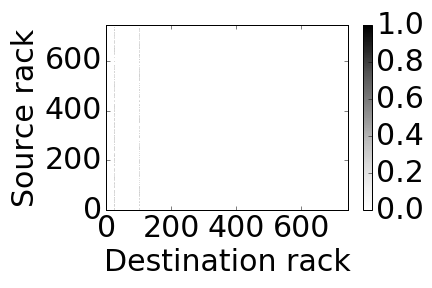
\includegraphics[width=0.3\linewidth]{pictures/ProjecToR1.png}
	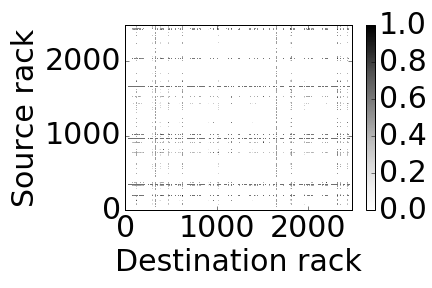
\includegraphics[width=0.3\linewidth]{pictures/ProjecToR2.png}
	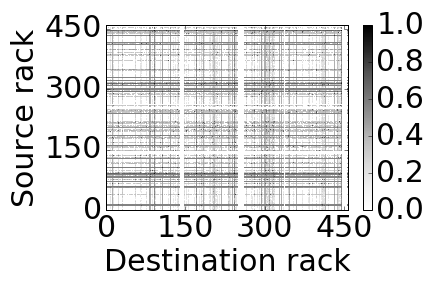
\includegraphics[width=0.3\linewidth]{pictures/ProjecToR3.png}
	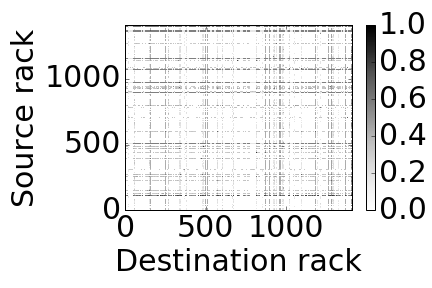
\includegraphics[width=0.3\linewidth]{pictures/ProjecToR4.png}
	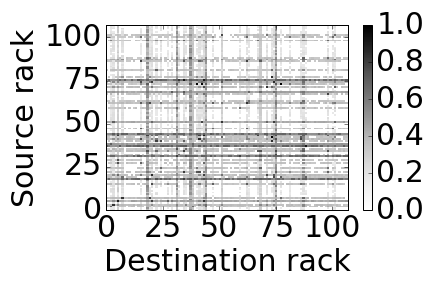
\includegraphics[width=0.3\linewidth]{pictures/ProjecToR5.png}
	\caption{Microsoft adattárház adatok klaszterenként}
	\label{microsoft-clasters}
\end{figure}

Amint a \ref{microsoft-clasters} ábrán látható, a kommunikáció főleg megadott szerverek között történik.
Korábban már említve volt, az adattárházak jelenleg a legrosszabb esetre vannak tervezve, hogy bármelyik két szerver tudjon kommunikálni.
Az ábrán látszik, hogy melyik szerverek között nem szükséges feltétlen direkt kapcsolatot kiépíteni, hanem elég egy már meglévő közvetett útvonalat használni, ahol kicsi a torlódás.
Az ilyen hálózat megtervezéséhez először szükségünk van arra, hogy tudjuk milyen tervezési stratégiák vannak és, hogy az adattárházak milyen topológiával rendelkeznek jelenleg.

\subsection{Hálózat tervezési stratégiák}

\begin{itemize}
	\item A technika fejlődésével elérhetővé váltak eszközök arra, hogy egy adott hálózatot újra konfiguráljunk, attól függően milyen terhelés éri
	\begin{itemize}
		\item pl, korábbi kommunikációs minták alapján
	\end{itemize}
	\item Két fő optimalizációs lehetőség van, legyen rövid az út (a) vagy legyen minimális a torlódás (b)
	\item A cikk bemutat egy módszert arra, hogy lehet mindkettőre majdnem optimális megoldást adni egyszerre (c)
\end{itemize}

\begin{figure}[h]
	\centering
	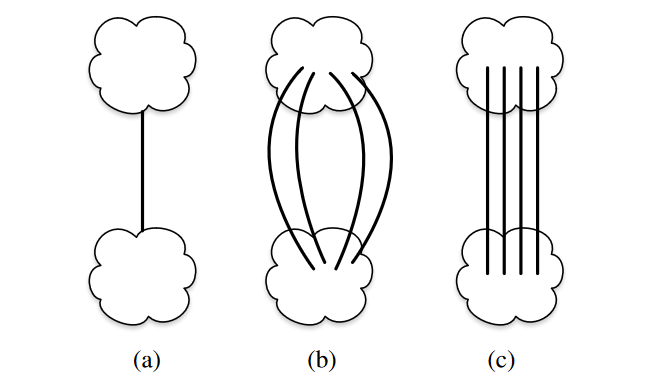
\includegraphics[width=8cm]{pictures/optimalshemes.png}
	\caption{Hálózat tervezési stratégiák, (a) rövid utakra való optimalizálás, (b) minimális torlódásra való optimalizálás, (c) mindkét esetre való optimalizálás}
	\label{network-strategies}
\end{figure}

\subsection{Adattárházak hálózati felépítése}

\begin{center}
	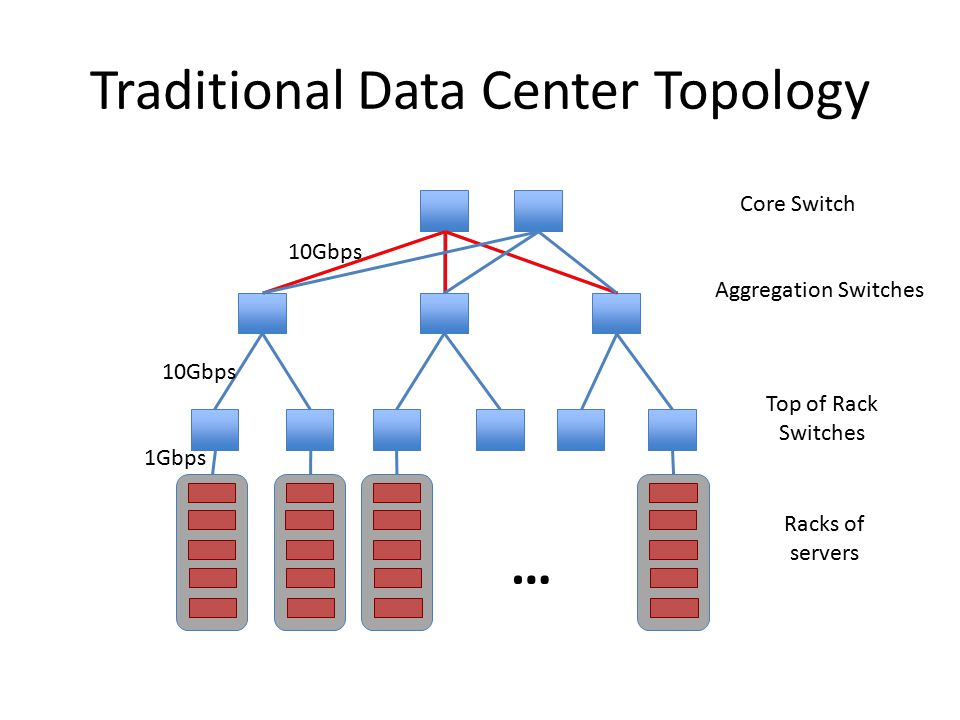
\includegraphics[width=0.7\linewidth]{pictures/Traditional+Data+Center+Topology.jpg}
\end{center}

\begin{itemize}
	\item Core switch
	\item Aggregation Swtiches
	\item Top of Rack Switches
	\item In-Rack Switches
\end{itemize}

\subsection{Újrakonfigurálás megvalósítása}

\begin{itemize}
	\item Átlag hálózatok statikusan vannak konfigurálva, nem  sok lehetőséget adva annak, hogy változtassunk 
	\begin{itemize}
		\item pl. Ethernet switchek
	\end{itemize}
	\item Optikai switchek már újra tudják konfigurálni magukat, de ezek "lassúak"
	\item Microsoft Research - ProjecToR\cite{ghobadi_projector:_2016}, lézer segítségével kiváltani az optikai swticheket, \ref{projector-fig} ábrán látható a maga az eszköz
	\begin{itemize}
		\item 12 $\mu s$ váltás idő ( 2500x gyorsabb mint egy optikai hálózati switch)
	\end{itemize}
	
	\begin{figure}[h]
		\centering
		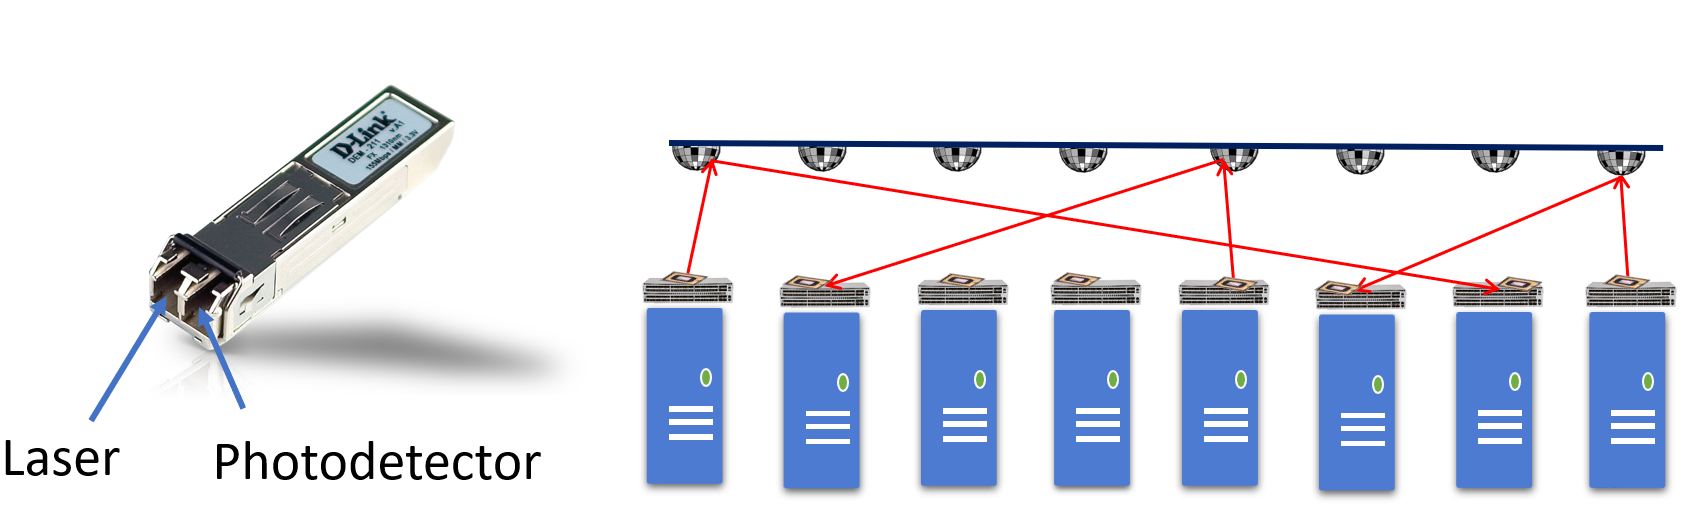
\includegraphics[width=0.9\linewidth]{pictures/laserswitch.png}
		\caption{ProjecToR}\label{projector-fig}
	\end{figure}
	
	
\end{itemize}

\section{Labor célja}

A labor célja a cikkben\cite{avin_demand-aware_nodate} bemutatott algoritmus implementálása, és annak alkalmazása különböző véletlenszerűen generált gráfokra. 
A kapott eredményeket össze lehet hasonlítani a megadott elméleti korlátokkal.

\section{Laborban megvalósított munka}

A labor ideje alatt elkészült egy keretrendszer, ami segítségével tesztelhető a szerzők által felvázolt algoritmus. 
A keretrendszer Python \cite{noauthor_python_nodate} nyelven íródott.
Egy véletlen gráfok generálására egy külső csomag lett használva \cite{noauthor_networkx_nodate}

\chapter{Modell}

\section{Forgalom igény tudatos hálózat tervezés probléma}

\begin{itemize}
	\item Vegyünk egy hálózatot meghatározott számú csomóponttal
	\item A hálózathoz tartozik egy demand mátrix, ami leírja a valószínűségét annak, hogy $i$ forrásból mekkora eséllyel lesz adat küldve $j$ célba
	\item A cél, hogy ezen adatból egy olyan hálózati séma készítése, ami kis torlódást és rövid utakat eredményez, ez mellett még skálázható is
\end{itemize}

\begin{figure}[h]
	\centering
	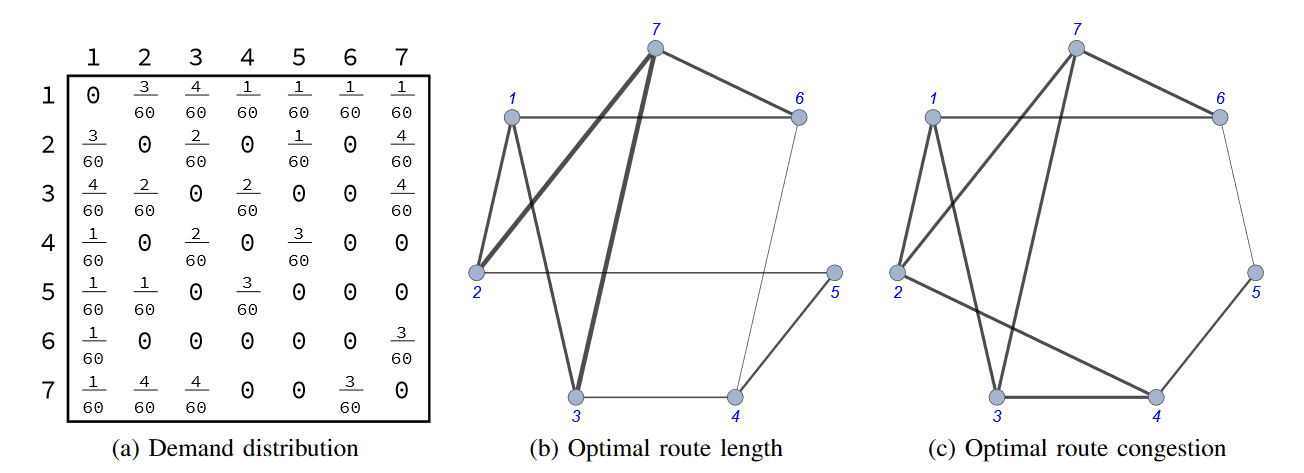
\includegraphics[width=14cm]{pictures/example.png}
	\caption{Forgalom igény tudatos hálózat tervezés probléma, (a) demand mátrix, (b) hálózat optimális úthosszra és (c) hálózat optimális torlódásra}
	\label{network-strategies}
\end{figure}

\section{Formális felírás}

\begin{itemize}
	\item Adott $N$ darab csúcspont  $V = \{1, ..., N\}$, és egy kommunikációs séma $M_D$ ami egy $N\times N$ mátrix
	\item A mátrix $(i, j)$ eleméhez tartozik egy $p(i, j)$ valószínűség, ahol $i$ a forrás csomópont és $j$ a cél
	\item A bemeneti mátrix ábrázolható egy irányított
	$G_D$ gráfban, ahol az élsúlyok a két pont közötti kommunikációs valószínűség
	\item Az algoritmus feltétele, hogy a mátrix ritka legyen
	\item Egy $N$ hálózatra a torlódást és az úthosszt útválasztási sémával fogjuk definiálni
	\item Egy útválasztási séma az $N$ hálózatra $\Gamma(N)$, ami $\Gamma_{uv}$ utak halmaza, ahol $(u, v)$ párok különböző utakat jelölnek
	\item $\Gamma_{uv}$ egy útsorozat, ami összeköti az $u$ pontot $v$ ponttal
\end{itemize}

\subsection{Torlódás}

\begin{mydef}
	A torlódást egy \(\Gamma(N)\) útválasztási sémán a \(D\) demand mátrix segítségével írjuk fel: \[C(D, \Gamma(N)) = \max_{e \in \Gamma(N)}  \sum_{e \in \Gamma(uv)} p(u,v) \]
\end{mydef}

\subsection{Úthossz}

\begin{mydef}
	Az átlag súlyozott úthosszt egy \(\Gamma(N)\) útválasztási sémán a \(D\) demand mátrix segítségével írjuk fel: \[L(D, \Gamma(N)) = \sum_{(u,v) \in D}  p(u,v)  \cdot d_{\Gamma(N)}(u, v) \] ahol a \(d_{\Gamma(N)}(u, v)\) az útvonal hosszát jelöli
\end{mydef}

\subsection{Skálázhatóság}

\begin{itemize}
	\item A hálózatot skálázhatóra kell tervezni, ezért meghatározunk egy \(\Delta\) konstans fokszámot, ami a maximális csatlakozások számát fogja meghatározni egy adott csomóponthoz
	\item \(N_\Delta\) jelölje az összes \(\Delta\) fokszámú gráfot, és elváruk, hogy \(N \in N_\Delta\)
\end{itemize}

\subsection{Optimális torlódás}

Az optimális torlódást egy  hálózatra, úgy határozzuk meg, hogy a csak a torlódást vesszük figyelembe számításkor \[C^*(D, \Delta) = \min_{N \in N_\Delta, \Gamma(N)} C(D, \Gamma(N))\]

\subsection{Optimális úthossz}

Az optimális úthosszt egy  hálózatra, úgy határozzuk meg, hogy a csak az úthosszt vesszük figyelembe számításkor \[L^*(D, \Delta) = \min_{N \in N_\Delta, \Gamma(N)} L(D, \Gamma(N))\]

\section{cl-DAN hálózat tervezése}
	
\begin{mydef}
	Adott egy \(D\) demand mátrix, és egy \(\Delta\) maximális fokszám, az \((\alpha, \beta)\)-cl-DAN hálózat tervezési probléma:
	\begin{itemize}
		\item Hogy tervezzünk egy olyan \(N \in N_\Delta\) hálózatot, és egy hozzá tartozó \(\Gamma(N)\) útválasztási sémát, ami közel optimális torlódásra és úthosszra is
	\end{itemize}

	Az algoritmus egy felső korlátot tud adni arra, hogy mennyivel fog eltérni a megoldás az optimálistól.
	\begin{itemize}
		\item Torlódásra: \(C(D, \Gamma(N)) \le \alpha \cdot C^*(D, \Delta) + \alpha'\)
		\item Úthosszra: \(L(D, \Gamma(N)) \le \beta \cdot L^*(D, \Delta) + \beta'\)
	\end{itemize}
	Az alfa vessző és béta vesszők olyan tényezők aki amik függetlenek a problémától
\end{mydef}

\section{EgoTree}

\begin{itemize}
	\item Az Egofa egy torlódásra és úthosszra optimalizált fa hálózat egy csomópontra nézve
	\item Az Egotree-t definiáljuk a következő módon, 
	
	\(EgoTree(s, \bar{p}, \Delta) \):
	\begin{itemize}
		\item \(s\) a forrás csomópont
		\item \(\bar{p}\) a szomszédainak eloszlásai
		\item \(\Delta\) fokszám
	\end{itemize}
	\item Ez közel optimális megoldást ad torlódásra és úthosszra
\end{itemize}

\begin{mytetel}
	Adott egy  \(\bar{p}\) frekvencia eloszlás az \(s\) forrás ponthoz, és adott egy \(\Delta\) fokszám, ekkor az \(EgoTree(s, \bar{p}, \Delta)\) egy \((\alpha, \beta)\)-cl-DAN a következő paraméterekkel:
	\begin{itemize}
		\item \(\alpha = \frac{4}{3}\)
		\item \(\beta = log^2(\Delta + 1)\)
	\end{itemize}
\end{mytetel}

\section{\(EgoTree(s, \bar{p}, \Delta)\) algoritmus}

\begin{enumerate}
	\item \(s\) a gyökér elem, \(\Delta\) fokszámmal, üres fa
	\item Rendezzük sorba \(\bar{p} = \{p1, p2, ..., p_k\}\) valószínűségeket csökkenő sorrendben
	\item Kezdjük rárakni a fára a csomópontokat, a gyökér elemre legfeljebb \(\Delta\) levél kerülhet
	\item Mikor elértük a \(\Delta\) levelet, a következő csomópontokat mindig a legkisebb összesített súlyú levélre kapcsolok rá, itt már legfeljebb két levele lehet minden fának
\end{enumerate}

\subsection{Algoritmus elemzése}

\begin{itemize}
	\item A kapott eredményben látható, hogy a maximális torlódás a legnagyobb súlyú élen van
	\item Minimalizálni ezt, lényegében egy időzítés probléma, hogy osszuk ki a munkákat \(\Delta\) processzornak, hogy minden leghamarabb kész legyen
	\item Erre az optimális algoritmus NP-nehéz, de van közelítő módszer
\end{itemize}

\subsection{Longest Processing Time (LPT)}

\begin{itemize}
	\item Először sorba rendezzük a feladatokat hossz szerint csökkenő sorrendben
	\item Ha van szabad processzor, akkor ahhoz rendeli a leghosszabb munkát
	\item Ha nincs akkor ahhoz a processzorhoz rendeli, ahol a legkevesebb ideig tart a munka
\end{itemize}
\begin{mytetel}
	Legyen \(\omega_L\) a maximum idő, mielőtt egy processzor befejezi az összes munkát a mohó LPT algoritmus szerint, és \(\omega_0\) az optimális, ekkor \[\frac{\omega_L}{\omega_0} \le \frac{4}{3} - \frac{1}{3\Delta}\]
\end{mytetel}

Ez az algoritmus polinom időben lefut

\begin{mylemma}
	Az \(EgoTree(s, \bar{p}, \Delta)\) ad egy \(\frac{4}{3}\) szorzóval nagyobb közelítést a minimális torlódásra az optimális \(\Delta\) fokú fához képest, ami kiszolgál \(\bar{p}\) frekvencia eloszlást egy adott \(s\) forrás csomópontra
\end{mylemma}

\begin{mylemma}
	Az \(EgoTree(s, \bar{p}, \Delta)\) ad egy \(log^2(\Delta + 1)\) szorzóval nagyobb közelítést a minimális úthosszra az optimális \(\Delta\) fokú fához képest, ami kiszolgál \(\bar{p}\) frekvencia eloszlást egy adott \(s\) forrás csomópontra
\end{mylemma}

\section{cl-DAN algoritmus}

\begin{mytetel}
	Legyen \(D\) egy szimmetrikus kommunikáció kéréseloszlás , ahol az átlag csúcs fokszáma \(\rho\), (azaz az élek száma \(\rho \cdot \frac{n}{2}\). Ekkor a maximum fokszám \(\Delta = 12\rho\), ehhez lehetséges generálni egy \((\alpha, \beta)\)-cl-DAN hálózatot, ahol:
	\begin{itemize}
		\item \(\alpha = 1 + (\frac{8}{9})\Delta\)
		\item \(\beta = 1 + 4log^2(\Delta + 1)\)
	\end{itemize}
\end{mytetel}
Konstans \(\rho\) esetén ez konstans közelítést ad a minimális torlódásra és az optimális úthosszra

\begin{enumerate}
	\item Felosszuk a hálózat csúcsait két halmazra, \(H\) - magas és \(L\) - alacsony fokszámúakra fele-fele arányban
	\begin{itemize}
		\item Az alacsony fokszámú csúcsok fokszáma legfeljebb \(2\rho\)
	\end{itemize}
	\item Megkeressük az összes olyan \((u, v)\) élt, ahol \(u\) és \(v\) is a magas fokszámú halmazba tartozik
	\item Az ilyen éleket a gráfban kiegészítjük egy segítő csomóponttal, \(l \in L\), az eredeti csomópontok között megszüntetjük az élt, és felveszünk két új élt \((u, l)\) és \((v, l)\)
	\begin{itemize}
		\item Minden segítő \(l\) csúcs választásakor egy még nem felhasználtat válasszunk az \(L\) halmazból
	\end{itemize}
	\item Meghatározunk egy mátrixot, ami első lépésben az eredeti
	\begin{itemize}
		\item Ahol segítő csomópontot vettünk fel, ott az útvonal hosszúhoz hozzá kell még adni az \(l\)-el való áthaladást is, és törölni kell az eredeti pontok közti élt
		\item Ezután elkészítjük a magas halmaz csúcsaira a \(T_u\) fát, ahol a valószínűségeket a mátrixból kiolvassuk, \(\Delta = 12\rho\) fokszámmal, ez közel optimális megoldást ad mindkét fel
	\end{itemize}
	\item Mivel \(u\) és \(v\) pontok közt egy \(l\) segítő csomópont van használva ezért \(T_u\) és \(T_v\) módosításra szorul. Alakítsuk át először \(T_u\)-t \(T'_u\)-ra
	\begin{itemize}
		\item Ha \(l \notin T_u\), \((p(u, l) = 0)\), akkor \(l\) átveszi \(v\) helyét \(T'_u\)-ban
		\item Ha \(l \in T_u\), \((p(u, l) > 0)\), akkor két lehetőségünk van:
		\begin{itemize}
			\item Ha \((p(u, l) > (p(u, v))\), akkor töröljük \(v\)-t a fából
			\item Ha \((p(u, l) \le (p(u, v))\), akkor \(l\) átveszi \(v\) helyét \(T'_u\)-ban
		\end{itemize}
		\item \(T'_v\) hasonlóan számítjuk ki, ezzel garantálva, hogy \(T'_u\) és \(T'_v\) közötti kommunikáció az \(l\) csomóponton keresztül fog áthaladni
	\end{itemize}
	\item Konstruáljuk meg az új N hálózatot, vegyük az előbb készített egofákat és vegyük az uniójukat, azaz húzzuk be az összes olyan élet amik szerepeltek a fákban
	\begin{itemize}
		\item     De mivel nem csak magas fokú csomópontok közt történhetett adatforgalom, ezért még vegyük hozzá az N hálózathoz azokat az éleket is, ahol mindkét csomópont alacsony fokszámú volt
	\end{itemize}
\end{enumerate}

\chapter{Megvalósítás}

\section{Keretrendszer}

A keretrendszer Python 3 nyelven íródott, és a Networkx külső csomag volt használva a véletlen gráfok generálására.
A példakód megtalálható futtatható hagyományos Python programként és Jupyter notebookban.  
Networkx csomag továbbá biztosít számunkra egy megjelenítési lehetőséget, amit a Jupyter notebookban tudunk legjobban kihasználni.



\section{Adatszerkezetek}

A modell alapját pár egyszerű alaptípus adja. Ezek rendre a következők:
\begin{itemize}
	\item \textbf{Vertex} - az általános gráf csúcspont
	\item \textbf{Node} - az \textit{Egófák} készítésekor használt csomópontok amik tartalmazzák a valószínűségét annak, hogy a forrás csomópont mekkora valószínűséggel fog kommunikálni a másik \textit{Node} csomóponttal
	\item \textbf{Edge} - az gráf csomópontjait reprezentáló él, ami \textit{Vertexet} vár paraméterként, és tárolja a valószínűséget, hasonlóan mint a \textit{Node}
	\item \textbf{Tree} - ami adja az alapját majd a útvonal tervezési sémának. A fának két fajtája lehet:
	\begin{itemize}
		\item \textbf{BinTree} - a kettő fokú fa
		\item \textbf{EgoTree} - a $\Delta$ fokú fa, ahol a gyökérnek legfeljebb $\Delta$ levele lehet, és a levelek pedig \textit{BinTree} típúsuak.
	\end{itemize}
	
\end{itemize}
	
\section{Modell}

A \textbf{Network} osztály valósítja meg az algoritmust, bemenete egy konfiguráció, kimenete egy útválasztási séma.
Ez mellett sok metaadatot is kiszámol a program amik között szerepel az átlag súlyozott úthossz és a torlódás.
A konfigurációban lehetőségünk van dinamikus delta fokszámot megadni, ezért metaadatok között szerepel a fokszám, amit az algoritmus használt számoláskor.
Az új hálózat létrehozásakor a csere lépéssorozat után, megváltozik a demand mátrix, ezért fontos, hogy a \(\Delta\) fokszámot ne haladjuk meg.
A metaadatok ezért tartalmazzák a delta fokszámot és a valós fokszámot, ami az algoritmus végeredménye lett.  
Ebből az adatból lehet következtetést levonni, hogy valóban megfelelő-e felső korlátja amit a szerzők adtak és lehet-e jobb felső korlátot adni. 

A bemeneti konfiguráció egy \textit{JSON} fájl, amit tartalmazhat több konfigurációt egyszerre.
Többféle módon lehet megadni konfigurációt attól függően milyen gráfot akarunk használni. 
Lehetőség van kézileg megadni a demand mátrixot vagy generálhatunk kétféle gráfot.
Véletlen gráfok amit tud generálni a program:
\begin{itemize}
	\item Erdős-Rényi gráf
	\item Barabási-Albert gráf
\end{itemize}

Egy minta konfiguráció, ami tartalmaz példát mind három esetre:

\begin{mintedJson}
{
  "config": [ {
	"graph": "erdos-renyi",
	"vertex_num": 11,
	"dan": null,
	"constant": 3
  }, {
	"graph": "barabasi-albert",
	"vertex_num": 11,
	"dan": 3,
	"m": 4
  }, {
	"graph": "manual",
	"vertex_num": null,
	"dan": 3,
	"demand": [
		[0, 3, 4, 1, 1, 1, 1],
		[3, 0, 2, 0, 1, 0, 4],
		[4, 2, 0, 2, 0, 0, 4],
		[1, 0, 2, 0, 3, 0, 0],
		[1, 1, 0, 3, 0, 0, 0],
		[1, 0, 0, 0, 0, 0, 3],
		[1, 4, 4, 0, 0, 3, 0]]	
	} ]
}
\end{mintedJson}

A konfigurációnak van három kötelező mezője, és a egy kiegészítő mező, attól függően, hogy melyik típusú gráfot választottuk. 

Kötelező mezők: 
\begin{enumerate}
	\item \textbf{graph} - a gráf típusa, három érték közül lehet választani:
	\begin{itemize}
		\item \textit{"erdos-renyi"} - Erdős-Rényi gráf 
		\item \textit{"barabasi-albert"} - Barabási-Albert gráf
		\item \textit{"manual"} - Kézzel megadott gráf
	\end{itemize}
	\item \textbf{vertex\_num} - A gráf csúcsainak száma. Ez nincs figyelembe véve kézzel adott gráf esetén, mivel meg van adva a demand mátrix és nem kell azt kigenerálni.
	\item \textbf{dan} - A Demand-Aware Network fokszámára ad megkötést. Értékek amit felvehet:
	\begin{itemize}
		\item \textit{null} - Alap beállítás szerint a cikkben ajánlott $12\rho$ fokszámot fogja használni
		\item \textit{12} - A megadott szám lesz a fokszám, példában most 12.
		\item \textit{"6d"} - A szám és egy "d" betűvel a végén hasonlóan működik mint az első eset, annyi különbséggel, hogy itt meg lehet adni, hogy mi legyen a $\rho$ szorzója, példa most $6\rho$
	\end{itemize}
\end{enumerate}

Konfiguráció függő mezők:
\begin{itemize}
	\item \textbf{constant} - \textit{Erdő-Rényi} gráf esetén a modell vár egy \(p\) valószínűséget ami annak a valószínűsége, hogy egy él be legyen húzva az új pontba, és ez független minden a korábban behúzott élektől. 
	A ritka mátrix eléréséhez a következő formulát használja a generáló algoritmus:  \[p = constant \cdot \frac{1}{vertex\_num}\]
	\item \textbf{m} - \textit{Barabási-Albert} gráf esetén a modell vár egy \(m\) számot, ami azt adja meg, hány olyan gráf ponthoz kell csatlakozzon az új, ami már eddig benne van a gráfban. 
	\item \textbf{demand} -  \textit{kézzel megadott} gráf esetén direkt módon megadható a mátrix, aminek a formája listák listája. 
	Figyeljünk arra, hogy négyzetes lehet csak a demand mátrix!
\end{itemize}

\section{Kimenet}

Az program kimenete, az algoritmus által kiszámolt metrikák, átlag súlyozott úthossz és torlódás. 
Ha a rajzolás opció be van kapcsolva, akkor a kiindulási hálózat, az egófák és az új hálózat választási séma ki lesz rajzolva.

\begin{figure}[h]
	\begin{center}
		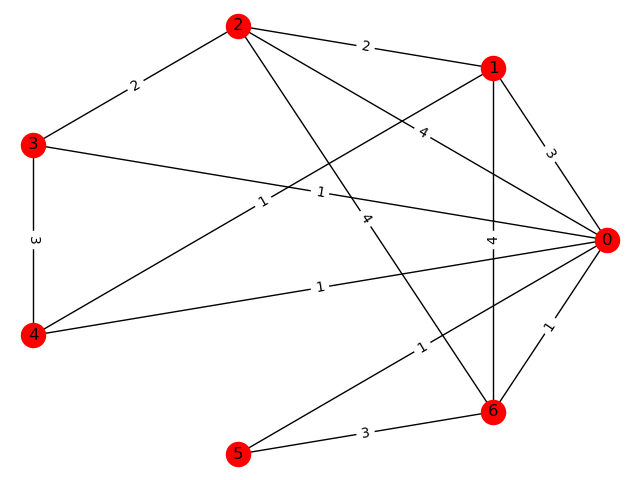
\includegraphics[width=0.49\linewidth]{pictures/starting_network.png}
		\caption{Kiindulási hálózat}
		\label{starting-network}
	\end{center}
\end{figure}

A \ref{starting-network} ábrán látható a bemeneti hálózat, aminek a demand mátrixa már a korábban fel lett írva. Az algoritmus ezek után a cl-DAN algoritmust használva, először elkészíti az egófákat \ref{ego-trees} ábra, majd végül az új hálózat választási sémát ami a \ref{routing-scheme} ábrán látható.

\begin{figure}[h]
	\begin{center}
		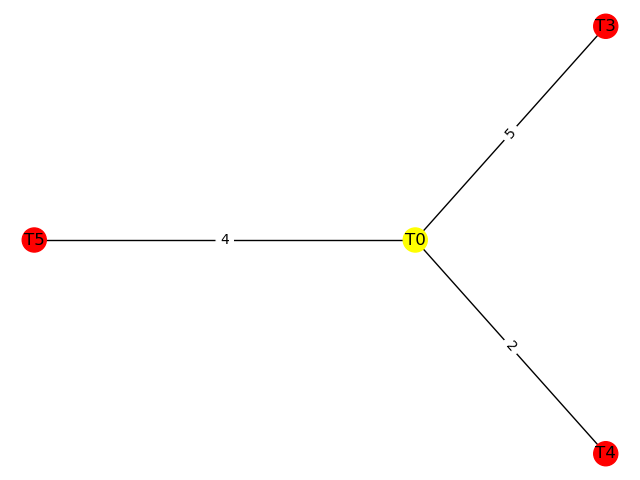
\includegraphics[width=0.40\linewidth]{pictures/egotree1.png}
		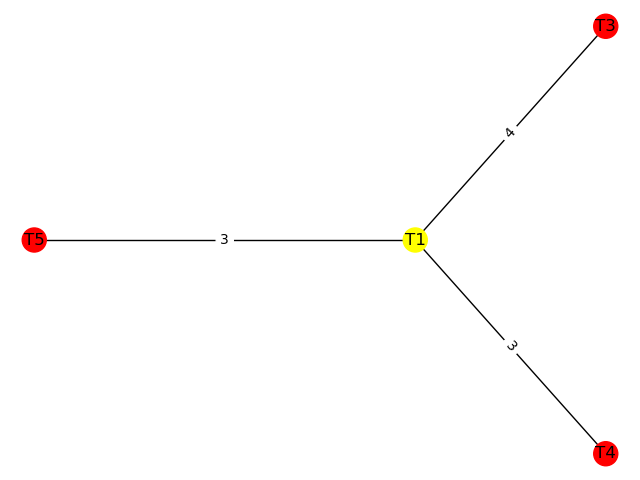
\includegraphics[width=0.40\linewidth]{pictures/egotree2.png}
		%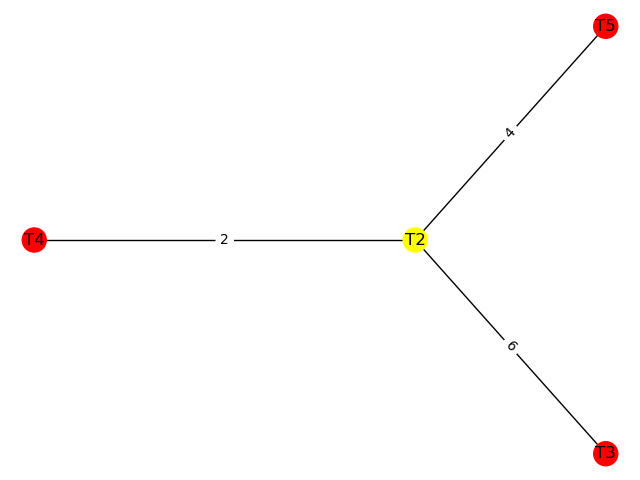
\includegraphics[width=0.40\linewidth]{pictures/egotree3.png}
		%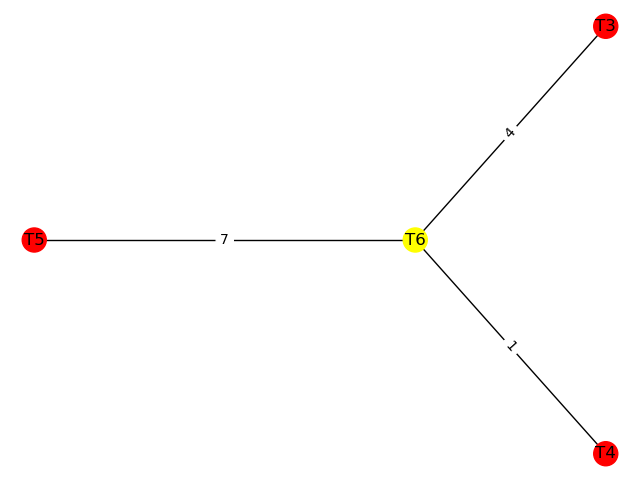
\includegraphics[width=0.40\linewidth]{pictures/egotree4.png}
		\caption{Egófák}
		\label{ego-trees}
	\end{center}
\end{figure}

A \ref{routing-scheme} ábrán látható gráfon pár extra információ megfigyelhető. 
Pirosra vannak festve a magas fokszámú csúcsok és zöldre az alacsony fokszámúak.
Az algoritmus fő célja az volt, hogy ne legyen egymással közvetlen kapcsolatban két magas fokszámú csúcs, azaz ne legyen két piros csúcs összekötve, és ez maradéktalanul teljesül is.
Két magas fokszú csúcs csak egy alacsony fokszámú segítő csúcson keresztül tud kommunikálni.
Fokszámok szempontjából a csúcsok rendben vannak, mivel nem haladják meg $\Delta$ fokszámot. 
A gráf esetén a delta \(\Delta = 12\rho = 12 \cdot \lceil\frac{25}{7}\rceil = 43  \).

\begin{figure}[h]
	\begin{center}
		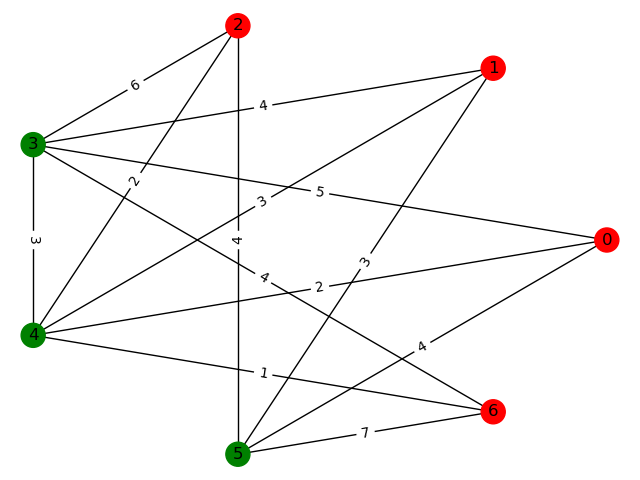
\includegraphics[width=0.49\linewidth]{pictures/new_network.png}
		\caption{Új hálózat}
		\label{routing-scheme}
	\end{center}
\end{figure}

\chapter{Teszt eredmények}

\section{Tesztelés menete}

A tesztelés során Erdős-Rényi gráfok voltak használva az egyszerű skálázhatóságból kifolyólag.
Három fő csoportba lehet a méréseket osztani a valószínűségi érték alapján, p = 0.25, p = 0.33 és p = 0.45.
A skálázhatóság tesztelésére különböző számú csúcspont volt használva, ezek rendre: 11, 15, 35, 50, 75, 100, 125, 150, 175 és 200.
A skálázhatósághoz még hozzátartozik a maximum fokszám, hogy mennyi gráf csúcs tud egyszerre kommunikálni, ezért az is meg van adva.
A valóságban van egy fizikai határ, hogy mennyi kliens tud csatlakozni egyszerre, ezért az értékek így lettek megválasztva, 3, 10, 16, 24 és 48.
A fenti paraméterek összes kombinációjára öt teszt lett futtat, majd azok átlagolva lettek.
Az adatok egy CSV fájlban lettek összegyűjtve, majd RapidMiner segítségével lett kiértékelve.

\section{Átlag súlyozott úthossz}

\begin{figure}[h]
	\begin{center}
		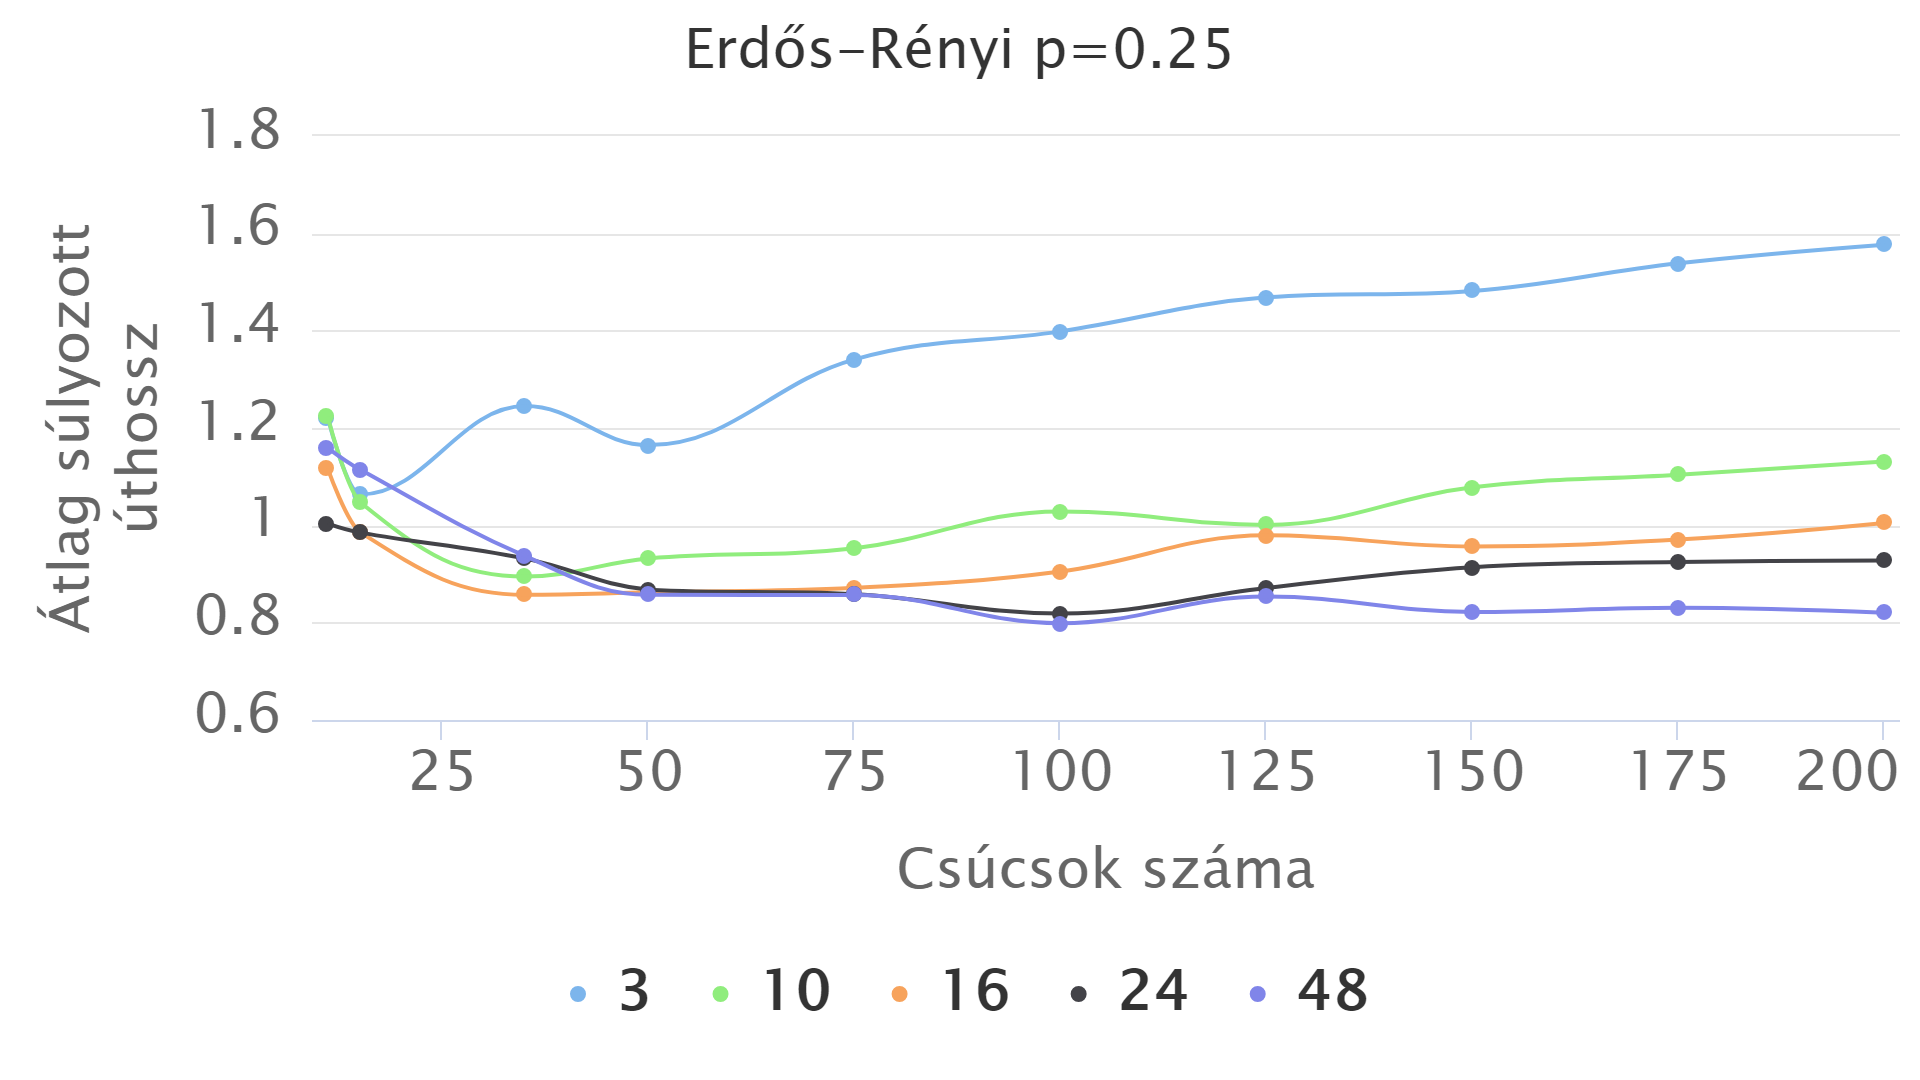
\includegraphics[width=0.40\linewidth]{pictures/constant_dan_ratio25_avg_route_len.png}
		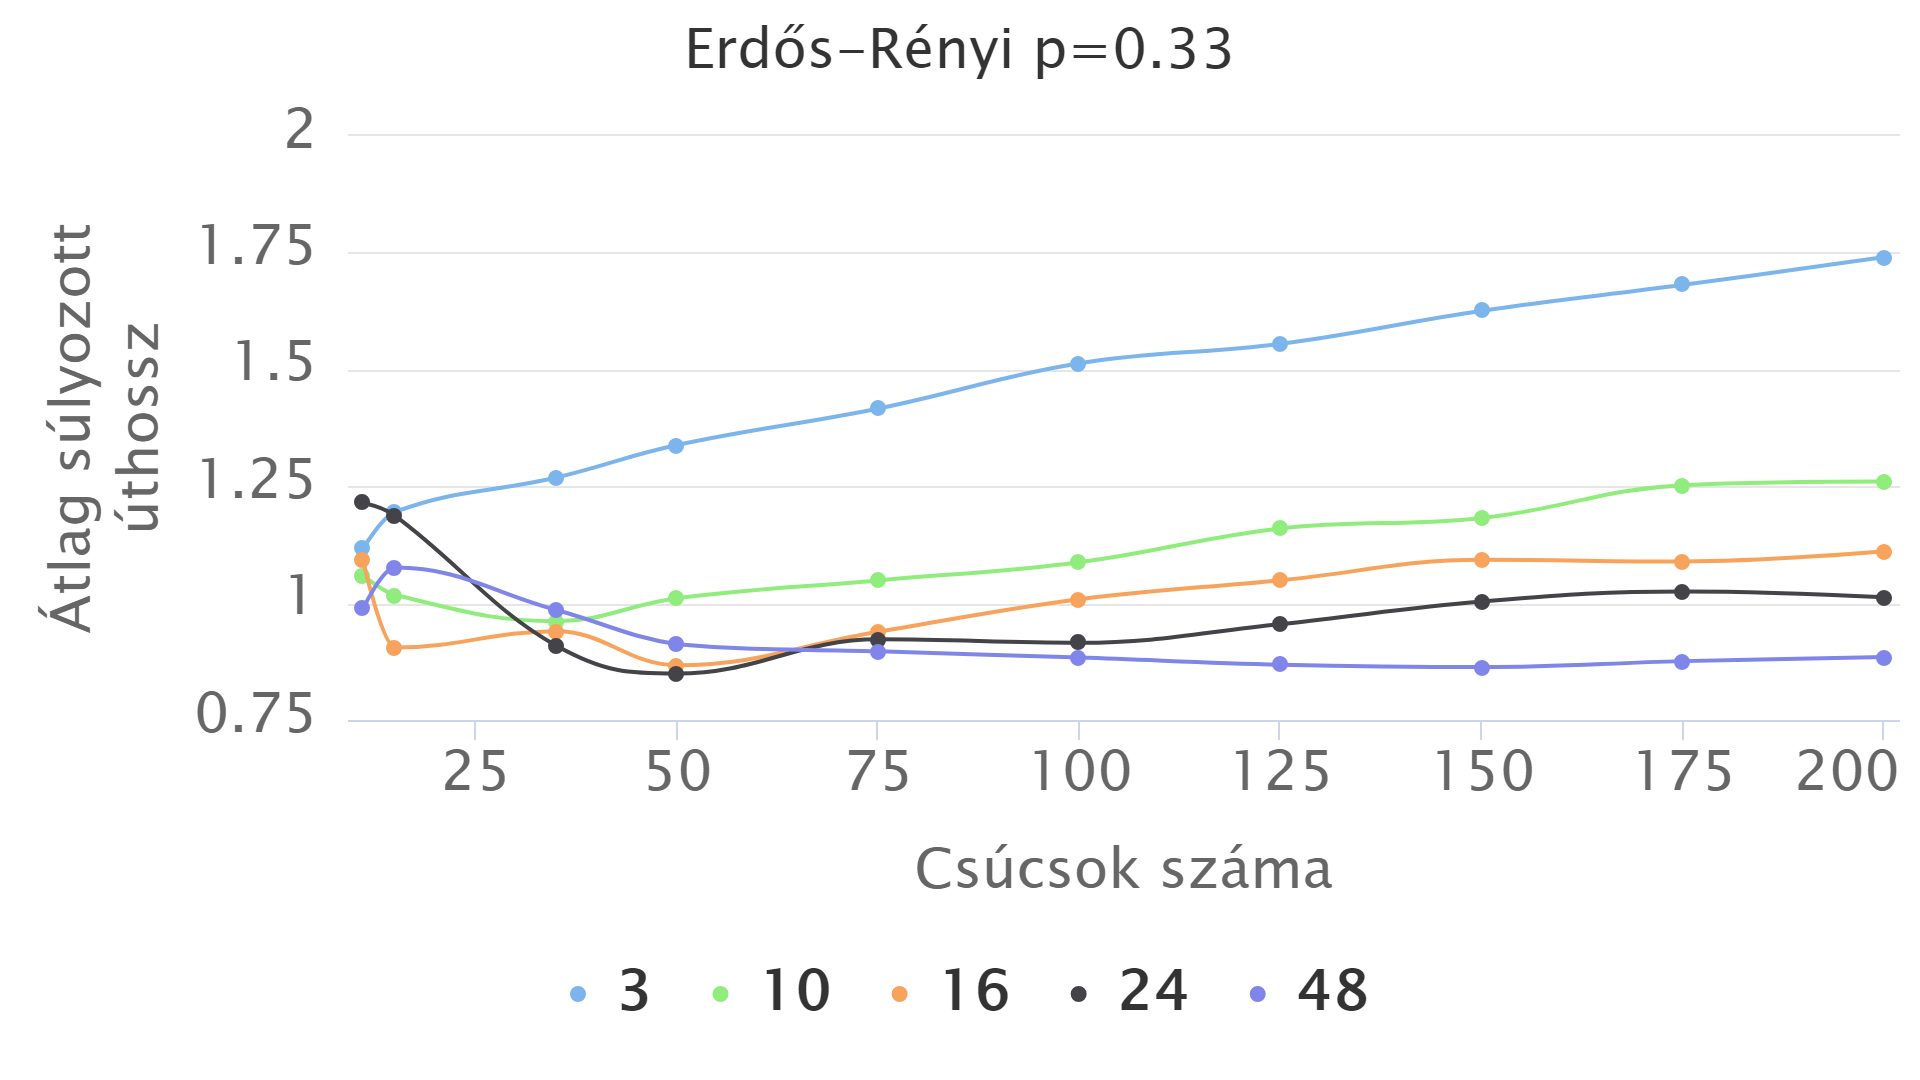
\includegraphics[width=0.40\linewidth]{pictures/constant_dan_ratio33_avg_route_len.png}
		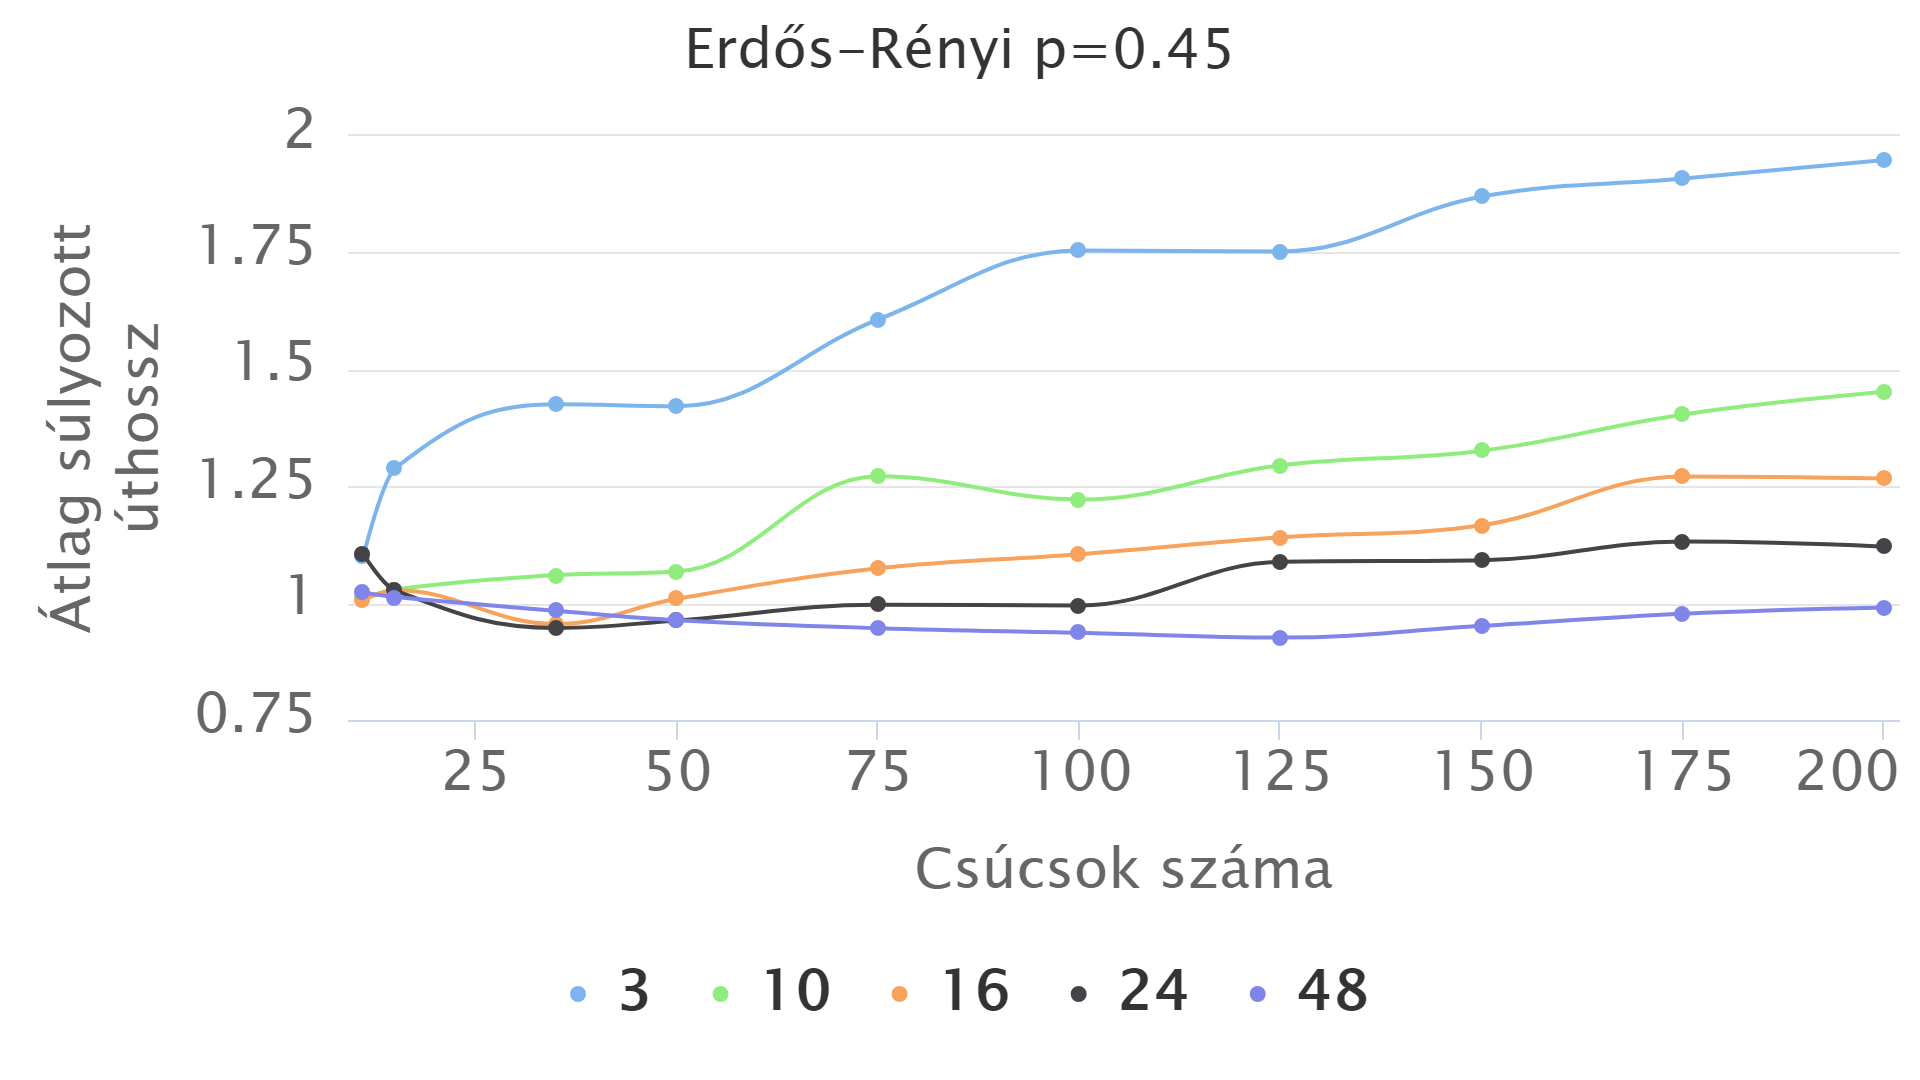
\includegraphics[width=0.40\linewidth]{pictures/constant_dan_ratio45_avg_route_len.png}
		\caption{Átlag súlyozott úthossz}
		\label{avg-len}
	\end{center}
\end{figure}


Az \ref{avg-len} ábrán látható az átlag súlyozott úthossz csúcspontok függvényében, és a delta fokszámra lebontva.
Az átlag súlyozott úthossz mind három esetben hasonlóan néz ki.
A konstans fokszám miatt egyértelműen látszik, hogy az értékek növekednek, kicsi delta esetén, pl. 3, ez nagyon jól megfigyelhető.
Az eredmények hasonlóak mind három esetben, a kitöltöttség növekedésével az értékek is növekednek, de a grafikon iránya nem változik.

\section{Átlag torlódás}

A \ref{congestion} ábrán látható az átlag torlódás. 
Hasonlóan mint az úthossznál a fő tényezők a csúcsok száma és az, hogy hogyan választjuk meg a fokszámot.
Ám ha megnézzük a két diagram irányát, két különböző dolgot mutatnak. 
A súlyozott úthossz növekedik ahogy hozzáveszünk további pontokat a hálózathoz, addig a torlódás mértéke közel exponenciálisan csökken.
Ennek egyszerű oka van, mert minél több csomópont közül tudunk választani, a terhelést egyre több pont között lehet elosztani és így a torlódás egészében csökken a hálózatban.

\begin{figure}[h]
	\begin{center}
		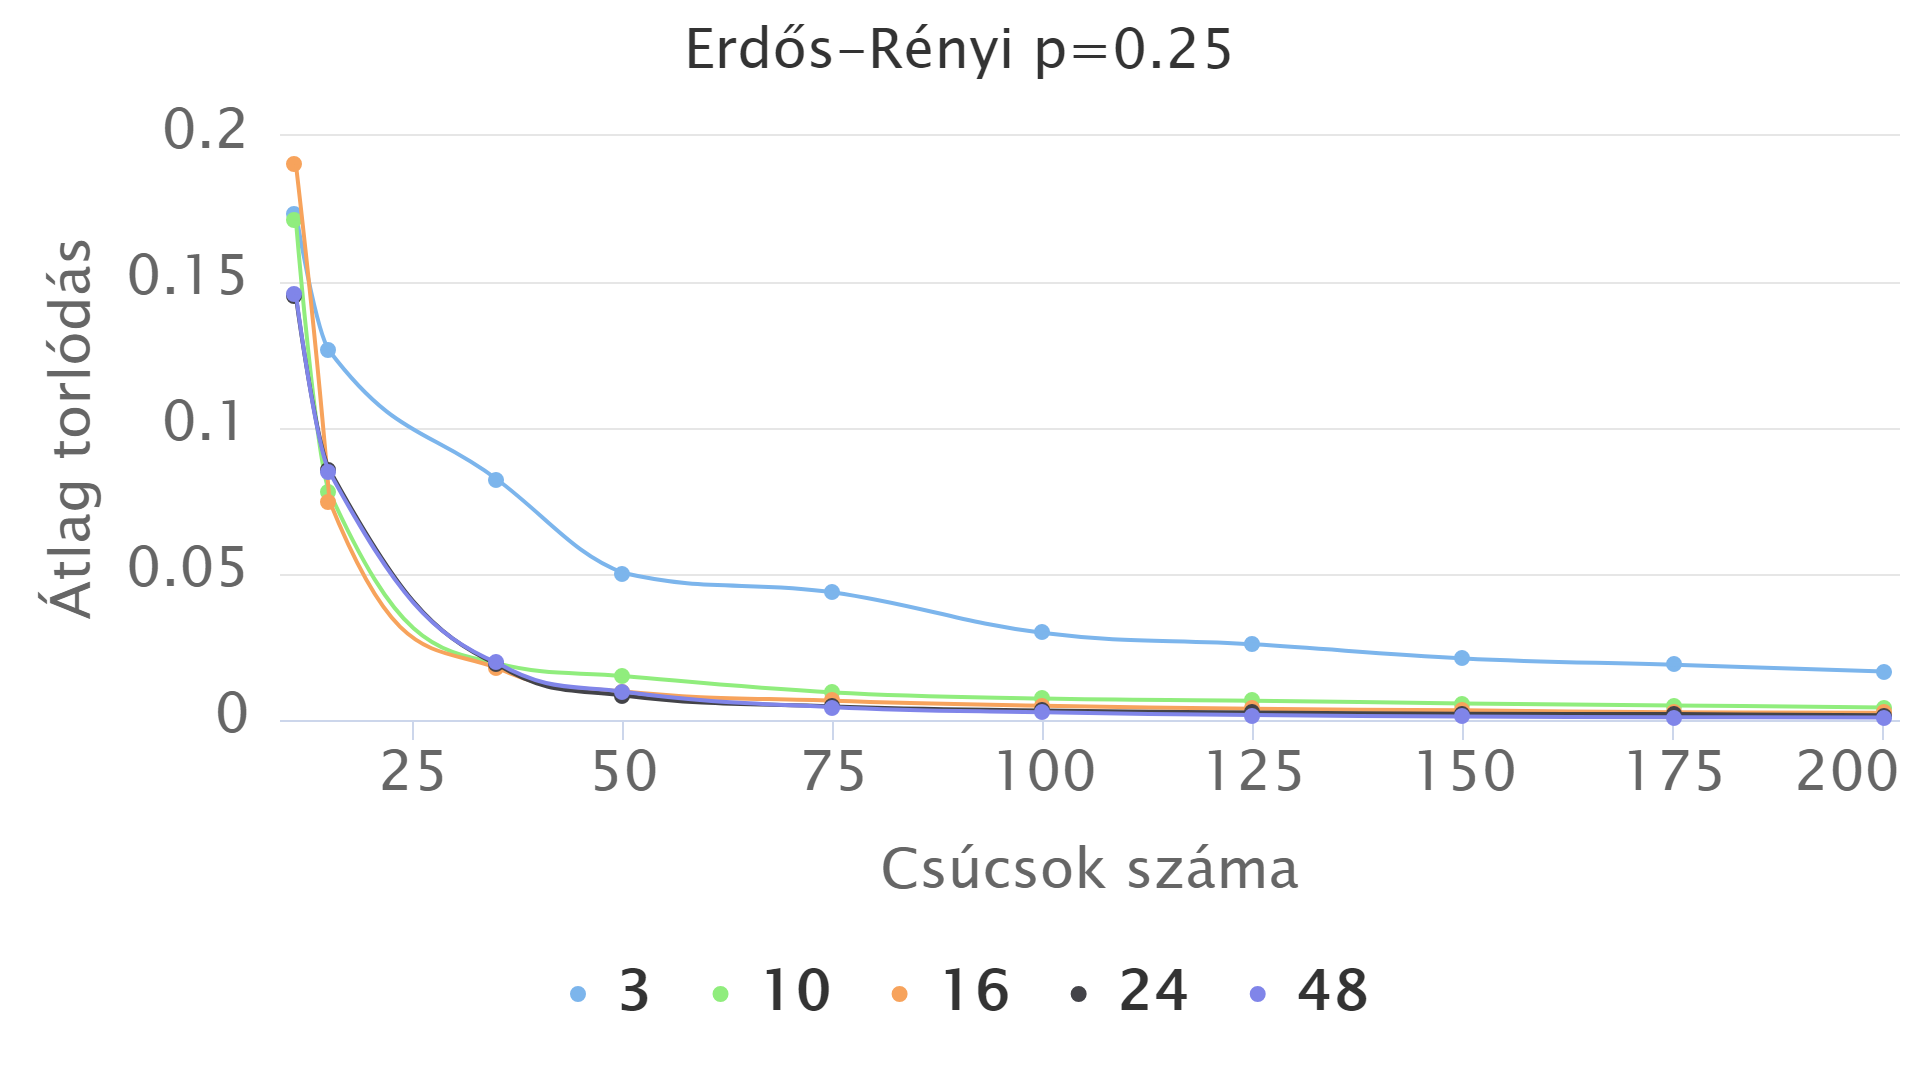
\includegraphics[width=0.40\linewidth]{pictures/constant_dan_ratio25_congestion.png}
		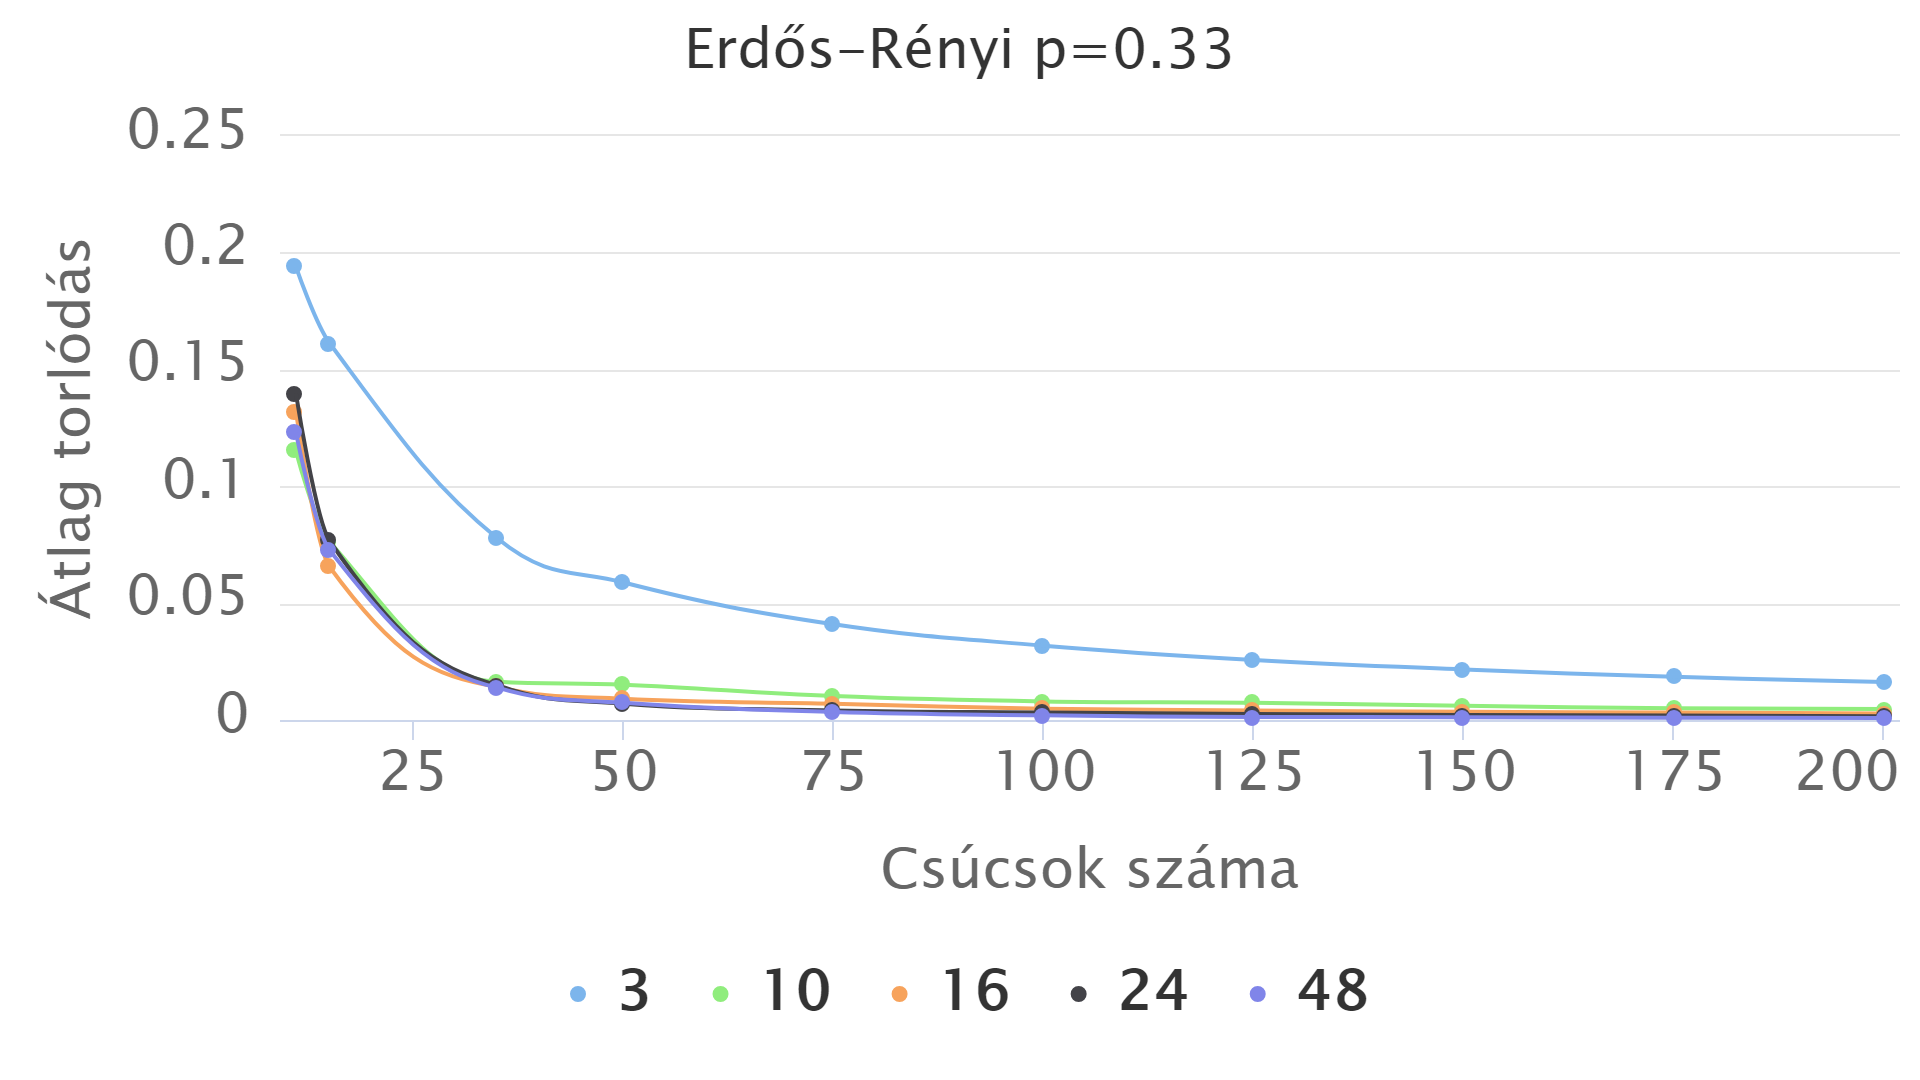
\includegraphics[width=0.40\linewidth]{pictures/constant_dan_ratio33_congestion.png}
		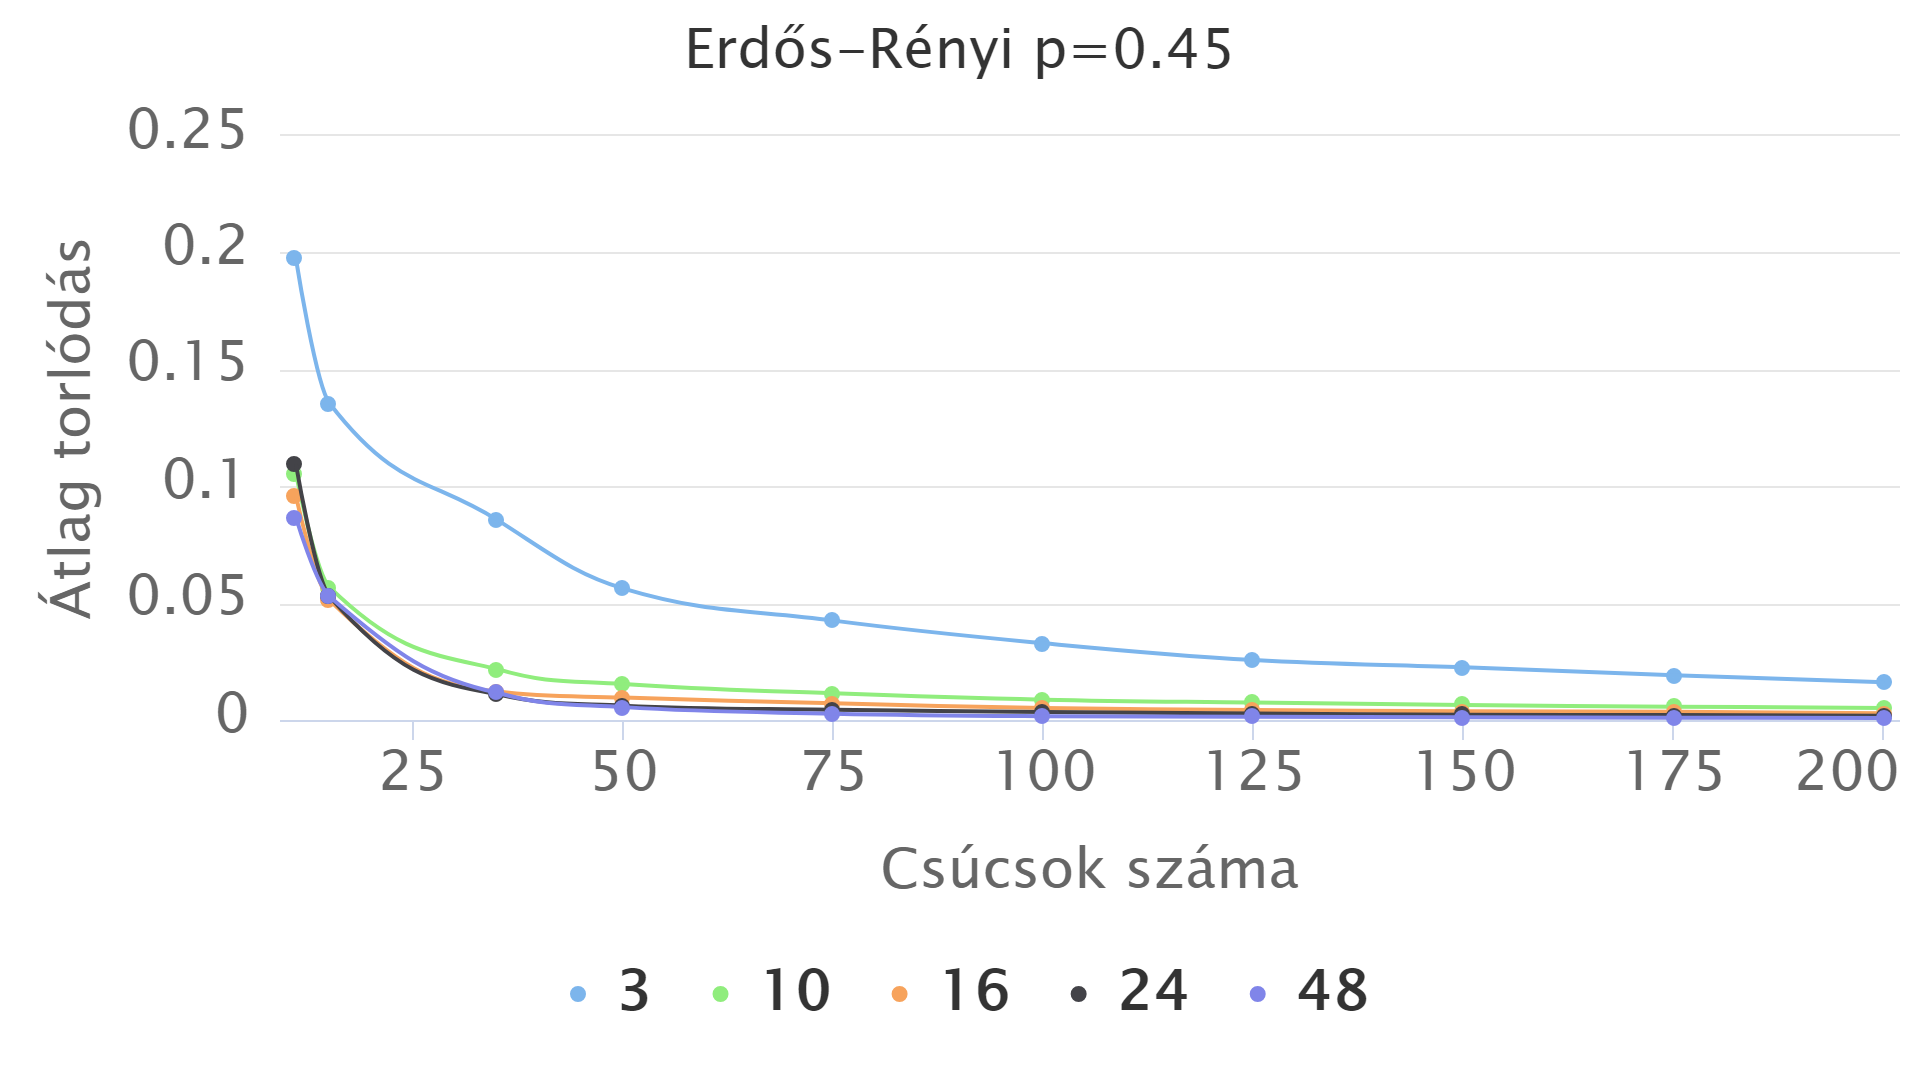
\includegraphics[width=0.40\linewidth]{pictures/constant_dan_ratio45_congestion.png}
		\caption{Átlag torlódás}
		\label{congestion}
	\end{center}
\end{figure}

\section{Fokszám}

A fentiekben már volt említve, hogy adott számú csomópontot használunk.
A cikkben szereplő felső korlátok az átlag fokszám függvényében van megadva, ami azt eredményezi, minden hálózatnak más $\Delta$ fokszám ad közel optimális megoldást.
Ez elméletben teljesül is, de ha megnézzük a \ref{delta} ábrát, rögtön észrevehető egy érdekes jelenség. 
A delta fokszám majdnem minden esetben nagyobb mint a csúcsok száma ami a hálózatban van.
Ez azt eredményezi, hogy minden csomópont közel két lépésből elérhető, és csak akkor van szükség az algoritmus újra rendező részére, 5. lépés, ha egy csomóponttal kommunikál több mint a fele pont a hálózatban.
Erre egy példa a 200 pontból álló hálózat, ami a képen látható, hogy már ha a $\Delta=4\rho$ a fokszámot annyi mint a pontok száma a hálózatban.

\begin{figure}[h]
	\begin{center}
		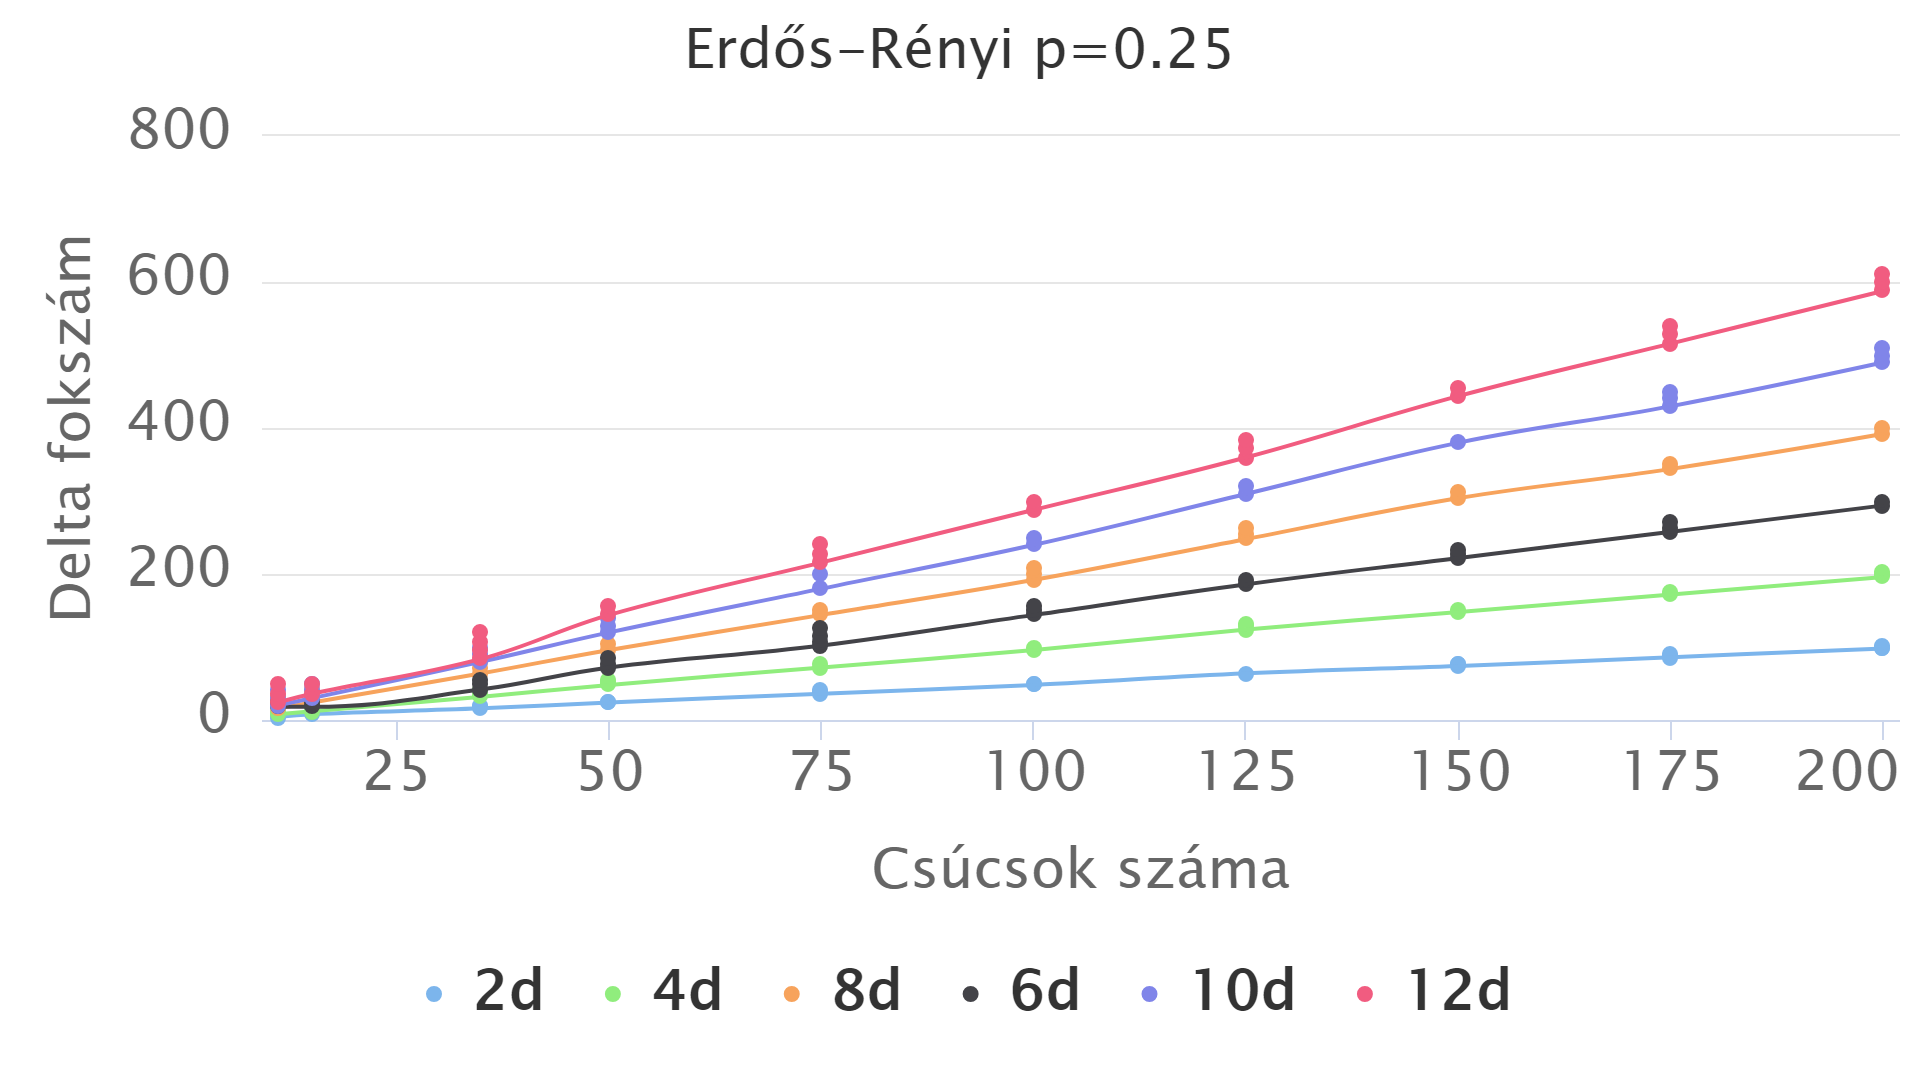
\includegraphics[width=0.40\linewidth]{pictures/constant_dan_ratio25_delta.png}
		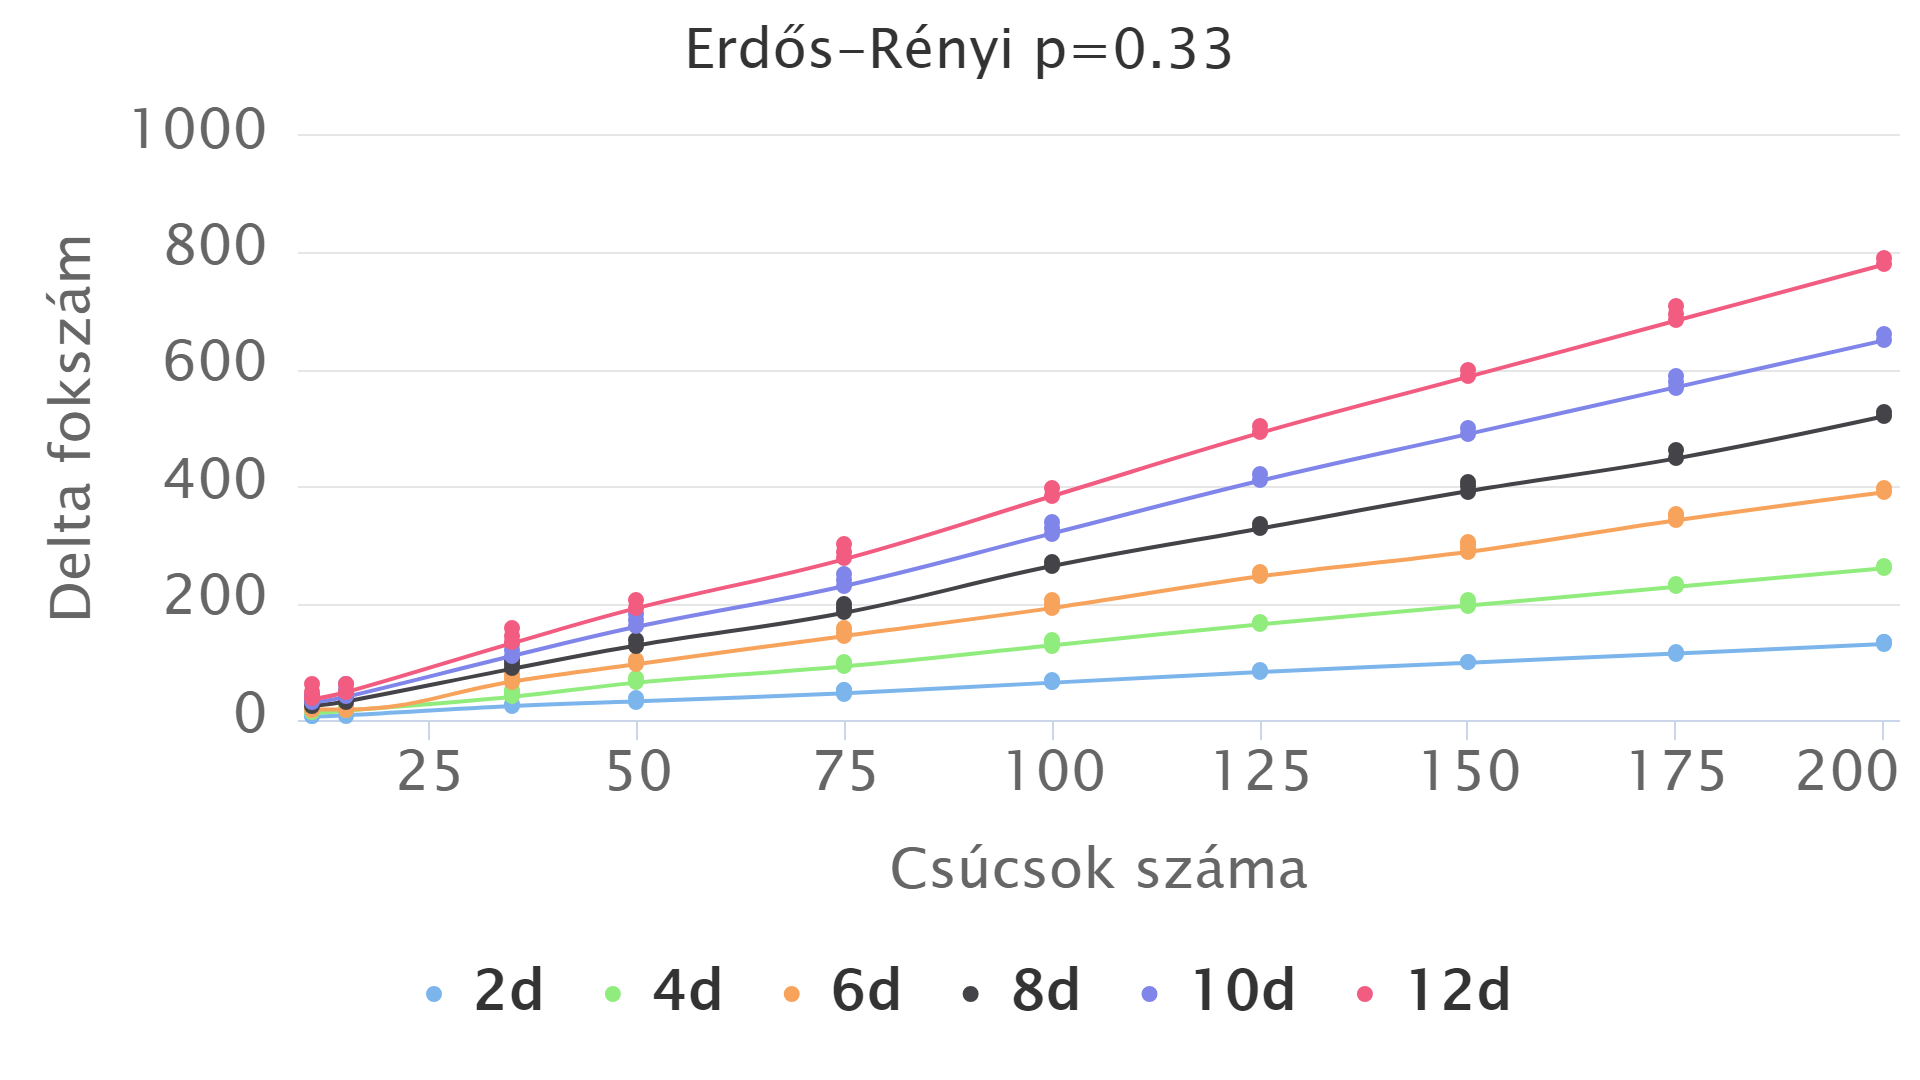
\includegraphics[width=0.40\linewidth]{pictures/constant_dan_ratio33_delta.png}		
		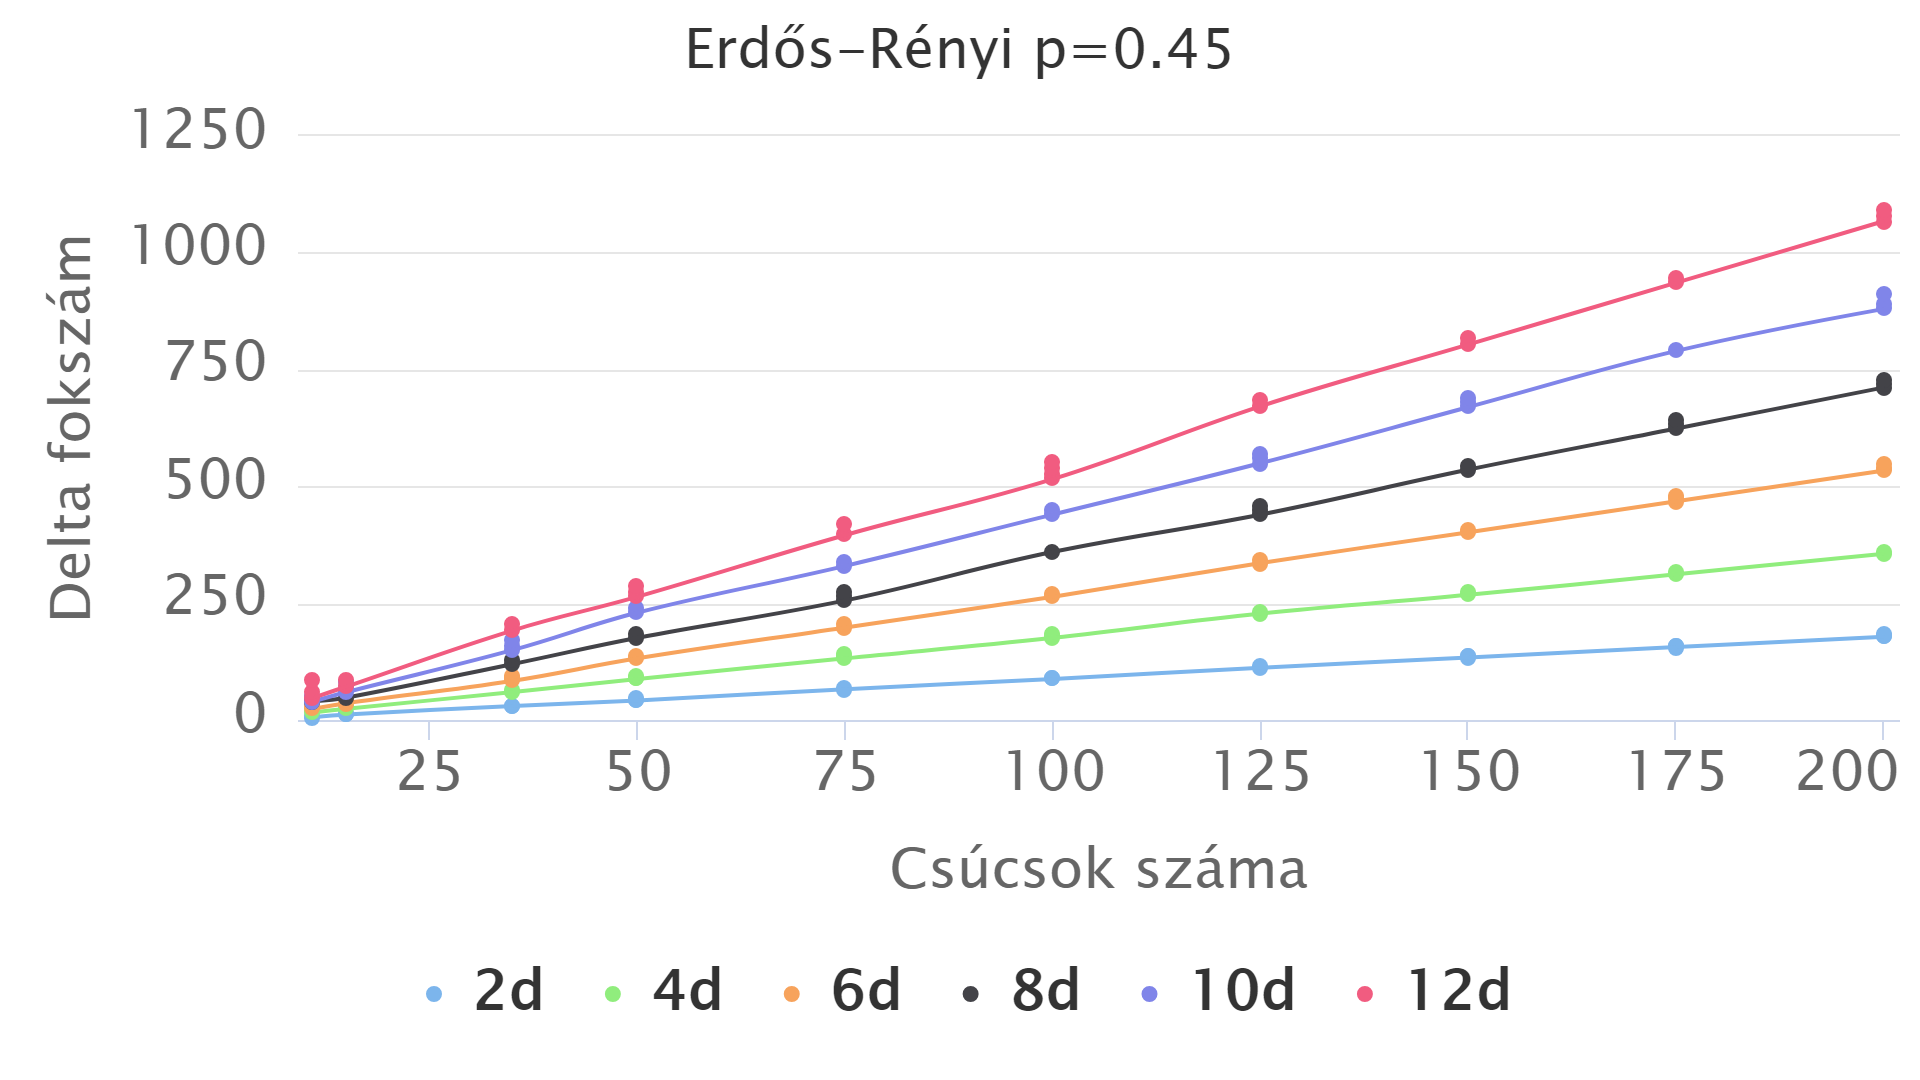
\includegraphics[width=0.40\linewidth]{pictures/constant_dan_ratio45_delta.png}
		\caption{Delta fokszám}
		\label{delta}
	\end{center}
\end{figure}

\chapter{Összefoglalás}

\section{Cikk eredménye}

Az technológia fejlődésével lehetőség nyílt arra, hogy a hálózatokat újrakonfiguráljuk futás időben.
A változó topológiának köszönhetően hatékonyabb lesz az adattárházak működése.
Az forgalom igény tudatos hálózatok tervezése körül jelenleg intenzív kutatás folyik ebből kifolyólag. 
A feldogozott cikk és a benne található algoritmus ad egy megoldást arra, hogy lehet ilyent tervezni.
Az algoritmus lényege, hogy a túlterhelt csomópontok között irányítsuk át forgalmat egy segéd csomóponton.
Ennek a megvalósítása az egófákkal van megadva, ahol lekorlátozzuk a maximális csatlakozások számát a jobban terhelt szerverekhez.
A szerzők által meghatároztak egy felső korlátot az átlag súlyozott úthosszra és torlódásra megadott fokszám mellett ami valóban megfelelő.


\section{Megjegyzések}

A teszt eredményekből látszik, hogy a $\Delta=12\rho$ fokszám egy nagyon magas korlát, mivel bőven túlmutat a rendelkezésre álló csúcsok számán. Feltételezhető, hogy ettől lehet jobb felső becslést is adni. 
Egy érdekes megfigyelés az algoritmus esetén, ha egy olyan fokszámot adunk meg, ami nem mutat túl a létező csúcspontok számán, hanem ellenkezőleg, elég szigorúra van véve.
Ilyenkor csak a magas fokszámú pontokra van garantálva, hogy a megadott fokszámú ponthoz csatlakoznak és ez nem fog teljesülni az alacsony fokszámúakra.
Egy ilyen eset legegyszerűbben akkor fordul elő, ha már telített a fokszáma a segítő pontnak magas fokú pontokkal. 
Mivel nem csak magas fokú csomópont fog kommunikálni egy segítővel, ezért még azokat is be kell húzni, mikor két segítő fog kommunikál, és ilyenkor nincs figyelve arra, hogy mi a jelenlegi fokszám. 

\bibliographystyle{abbrv}
\bibliography{refrences}

	
\end{document}